%% monografia.tex, fabiokepler
%% Copyright 2012-2013 by UNIPAMPA LaTeX group at http://bitbucket.org/unipampa/monografia-latex
%%
%% This work may be distributed and/or modified under the conditions of the LaTeX Project Public
%% License, either version 1.3 of this license or (at your option) any later version.
%% The latest version of this license is in
%%   http://www.latex-project.org/lppl.txt
%% and version 1.3 or later is part of all distributions of LaTeX version 2005/12/01 or later.
%%
%% Based on the example file abtex2-modelo-trabalho-academico.tex of the abntex2 package
%% (http://abntex2.googlecode.com/) and on the ppgccufmg 1.45beta2 class
%% (http://vilarneto.com/ppgccufmg,
%% http://www.dcc.ufmg.br/pos/alunos/modelodisstese.php
%% and http://www.dcc.ufmg.br/~mirella).
%%
%% Adapted for the Computer Science program at UNIPAMPA (http://www.unipampa.edu.br)
%% by Fabio Kepler (fabio@kepler.pro.br).
%%
%% Version 2.3 - 2013/03

% +++++++++++++++++++++++++++++++++++++++++++++++++++++++++++++++++++++++++++++++++++++++++++++++++
% Este modelo utiliza o pacote abnTeX2. Veja como instalá-lo em seu ambiente em
% http://abntex2.googlecode.com/.
% -------------------------------------------------------------------------------------------------
% abnTeX2: Modelo de Trabalho Acadêmico (tese de doutorado, dissertação de
% mestrado e trabalhos monográficos em geral) em conformidade com
% ABNT NBR 14724:2011: Informação e documentação - Trabalhos acadêmicos -
% Apresentação
% -------------------------------------------------------------------------------------------------
% Normas institucionais utilizadas:
% http://porteiras.r.unipampa.edu.br/portais/sisbi/manual-de-normalizacao/
% +++++++++++++++++++++++++++++++++++++++++++++++++++++++++++++++++++++++++++++++++++++++++++++++++

\documentclass[12pt,openright,twoside,a4paper]{abntex2}    % frente e verso
%\documentclass[12pt,oneside,a4paper]{abntex2}            % apenas frente

% +++++++++++++++++++++++++++++++++++++++++++++++++++++++++++++++++++++++++++++++++++++++++++++++++
% PACOTES
% -------------------------------------------------------------------------------------------------
% Pacotes fundamentais
\usepackage{cmap}           % Mapeamento de caracteres especiais no PDF
\usepackage{lmodern}        % Usa fonte Latin Modern
\usepackage[T1]{fontenc}    % Seleção de codificação de fonte
\usepackage[utf8]{inputenc} % Codificação do arquivo (conversão automática dos acentos)
\usepackage[brazil]{babel}  % Idioma para hifenização e tradução de vários elementos
\usepackage{makeidx}        % Criação de índice
\usepackage{hyperref}       % Formatação do índice
\usepackage{lastpage}       % Usado pela Ficha catalográfica
\usepackage{indentfirst}    % Indenta o primeiro parágrafo de cada seção
\usepackage[usenames,dvipsnames]{xcolor}  % Controle das cores (com nomes)
\usepackage{graphicx}       % Inclusão de gráficos
\usepackage{booktabs}       % Formatação de tabelas
% -------------------------------------------------------------------------------------------------
% Para citações
\usepackage[brazilian,hyperpageref]{backref} % Páginas com as citações na bibliografia
\usepackage[alf]{abntex2cite} % Citações padrão ABNT (alfanumérico)
% -------------------------------------------------------------------------------------------------
% Pacotes opcionais
\usepackage{nomencl}        % Para criar uma lista de símbolos
\usepackage{acro}           % Para usar acrônimos e abreviaturas
\usepackage{tikz}           % Para fazer figuras, diagramas e gráficos integrados e elegantes
\usepackage{pgfplots}       % Usa o pacote tikz para fazer gráficos muito melhores que os do Excel
\usepackage{pgfplotstable}  % Para gerar tabelas automaticamente a partir de arquivos com dados
\usepackage{filecontents}   % Para colocar o conteúdo de um arquivo dentro de um arquivo tex
\usepackage{todonotes}      % Para criar anotações durante o desenvolvimento do texto
%\usepackage{multirow}       % Permite fazer tabelas com múltiplas linhas
%\let\newfloat=\undefined    % Workaround para usar o pacote algorithm
%\usepackage{algorithm}      % Para escrever algoritmos
%\usepackage{clrscode}       % Para escrever algoritmos
%\usepackage{clrscode3e}     % Para escrever algoritmos; mais simples que os pacotes acima
\usepackage{pdfpages}        % Para incluir a folha de aprovação assinada em PDF
\usepackage{amsmath}
\usepackage{amsfonts}
\usepackage{subcaption} 

% -------------------------------------------------------------------------------------------------
% Configurações de pacotes
% -------------------------------------------------------------------------------------------------
% Configurações do pacote backref
% Usado sem a opção hyperpageref de backref
\renewcommand{\backrefpagesname}{Citado na(s) página(s):~}
% Texto padrão antes do número das páginas
\renewcommand{\backref}{}
% Define os textos da citação
\renewcommand*{\backrefalt}[4]{
    \ifcase #1 %
        Nenhuma citação no texto.%
    \or
        Citado na página #2.%
    \else
        Citado #1 vezes nas páginas #2.%
    \fi}%
% -------------------------------------------------------------------------------------------------
% Configurações de aparência do PDF final
\definecolor{blue}{RGB}{41,5,195}
% \definecolor{webgreen}{rgb}{0,.5,0}
% Metainformações do PDF e cores dos links
\hypersetup{
  portuguese,
  %backref=true,
  %pagebackref=true,
  %bookmarks=true,             % show bookmarks bar?
  %bookmarksnumbered=true,
  bookmarksdepth=4,
  pdftitle={\@title},
  pdfauthor={\@author},
  pdfsubject={\imprimirpreambulo},
  pdfkeywords={UNIPAMPA}{Computação}{UNIPAMPA}{abntex}{TCC},
  %pdfproducer={LaTeX with abnTeX2},     % producer of the document
  pdfcreator={\@author},
  colorlinks=true,           % false: boxed links; true: colored links
  linkcolor=blue,            % color of internal links
  citecolor=blue,            % color of links to bibliography
  filecolor=magenta,         % color of file links
  urlcolor=blue
}
%   linktocpage,
%   colorlinks,
%   citecolor=webgreen,
%   urlcolor=Maroon,
%   linkcolor=RoyalBlue,
%   filecolor=black,
% -------------------------------------------------------------------------------------------------
% Espaçamentos entre linhas e parágrafos
% O tamanho do parágrafo é dado por
\setlength{\parindent}{1.3cm}
% Controle do espaçamento entre um parágrafo e outro
\setlength{\parskip}{0.2cm} % tente também \onelineskip
% Controles do espaçamento entre linhas
%\OnehalfSpacing       % espaçamento um e meio (padrão);
%\DoubleSpacing        % espaçamento duplo
%\SingleSpacing        % espaçamento simples
% -------------------------------------------------------------------------------------------------
% Para o pacote de acrônimos
\acsetup{hyperref=true,index=true} %first-style=short}
% -------------------------------------------------------------------------------------------------
% Para o pacote tikz, pgfplots e pgfplotstable
\usetikzlibrary{arrows,chains,matrix,positioning,decorations.pathreplacing,calc}
% -------------------------------------------------------------------------------------------------
% Para poder usar subfiguras e subtabelas
\newsubfloat{figure}
\newsubfloat{table}
\providecommand*{\subfigureautorefname}{\figureautorefname}
% +++++++++++++++++++++++++++++++++++++++++++++++++++++++++++++++++++++++++++++++++++++++++++++++++


% +++++++++++++++++++++++++++++++++++++++++++++++++++++++++++++++++++++++++++++++++++++++++++++++++
% Informações de dados para CAPA e FOLHA DE ROSTO
% -------------------------------------------------------------------------------------------------
\titulo{Modelo para Trabalho de Conclusão de Curso}
\autor{Marcos Vinícius Treviso}
\local{Alegrete}
\data{2015}
\orientador{Fábio Natanael Kepler}
\coorientador{} % Se houver
\instituicao{Universidade Federal do Pampa}
\tipotrabalho{Projeto de Trabalho de Conclusão de Curso} % Para TCC I
% \tipotrabalho{Trabalho de Conclusão de Curso~} % Para TCC II
% O preambulo deve conter o tipo do trabalho, o objetivo, o nome da instituição e a área de concentração
\preambulo{\imprimirtipotrabalho apresentado ao Curso de Graduação em Ciência da
           Computação da Universidade Federal do Pampa como requisito parcial para a obtenção do
           título de Bacharel em Ciência da Computação.}
% +++++++++++++++++++++++++++++++++++++++++++++++++++++++++++++++++++++++++++++++++++++++++++++++++

% -------------------------------------------------------------------------------------------------
% Compila o indice
\makeindex
% Compila a lista de abreviaturas e siglas
% Para funcionar, o seguinte comando deve ser executado:
% makeindex ARQUIVO_PRINCIPAL.nlo -s nomencl.ist -o ARQUIVO_PRINCIPAL.nls
\makenomenclature
% -------------------------------------------------------------------------------------------------

% -------------------------------------------------------------------------------------------------
% Abreviaturas (definido pelo parâmetro 'class')
\DeclareAcronym{fig}{
  short = Fig.,
  long  = Figura,
  class = abreviaturas
}
% -------------------------------------------------------------------------------------------------
% Acrônimos/Siglas (definido pelo parâmetro 'class')
\DeclareAcronym{tcc}{
  short = TCC,
  long  = Trabalho de Conclusão de Curso,
  long-plural-form = Trabalhos de Conclusão de Curso,
  class = acronimos
}

\DeclareAcronym{pos}{
  short = POS,
  long  = Part-of-speech,
  class = acronimos
}

\DeclareAcronym{pln}{
  short = PLN,
  long  = Processamento de Linguagem Natural,
  class = acronimos
}

% -------------------------------------------------------------------------------------------------
% Nomenclaturas/Símbolos
\nomenclature{$A_i$}{Área do $i^{esimo}$ componente}
\nomenclature{$\mathcal{T}$}{Conjunto de trabalhos de TCC}
\nomenclature{$X$}{Dados de entrada ou \textit{features}}
\nomenclature{$Y$}{Dados de saída}
\nomenclature{$X_j^{(i)}$}{O valor da \textit{feature} \textit{j} no i-ésimo exemplo de treinamento}
\nomenclature{$X^{(i)}$}{O vetor coluna de todas as \textit{features} no i-ésimo exemplo de treinamento}
\nomenclature{$m$}{Número de exemplos de treinamento}
\nomenclature{$n$}{$|X^{(i)}|$, o número de \textit{features}}
\nomenclature{$(x, y)$}{Um exemplo de treinamento}
\nomenclature{$(X^{(i)}, Y^{(i)})$}{O i-ésimo exemplo de treinamento}
\nomenclature{$\theta$}{Parâmetros a serem aprendidos}

% -------------------------------------------------------------------------------------------------
% Inclui alguns ajustes finos para que fique de acordo com o Manual de Normatização
% Pequenos consertos e ajustes para que fique de acordo com o Manual de Normatização 2011.

% ---
% Impressão da Capa
\renewcommand{\imprimircapa}{%
  \begin{capa}%
    \center
    \vspace*{1cm}
    {\ABNTEXchapterfont\large\imprimirinstituicao}
    \par
    {\ABNTEXchapterfont\large\imprimirautor}

    \vspace*{\fill}
    {\ABNTEXchapterfont\bfseries\LARGE\imprimirtitulo}
    \vspace*{\fill}

    {\large\imprimirlocal}
    \par
    {\large\imprimirdata}

    \vspace*{1cm}
  \end{capa}
}
% ---


% ---
% Impressão da Folha de Rosto
\makeatletter
\renewcommand{\folhaderostocontent}{
  \begin{center}

    {\ABNTEXchapterfont\large\imprimirautor}

    \vspace*{\fill}%\vspace*{\fill}
    {\ABNTEXchapterfont\bfseries\Large\imprimirtitulo}
    \vspace*{\fill}

    \abntex@ifnotempty{\imprimirpreambulo}{%
      \hspace{.45\textwidth}
      \begin{minipage}{.5\textwidth}
        {\SingleSpacing
        \imprimirpreambulo}

        \vspace*{1em}
        \imprimirorientadorRotulo~\imprimirorientador\par

        \abntex@ifnotempty{\imprimircoorientador}{%
          \vspace*{1em}
          \imprimircoorientadorRotulo~\imprimircoorientador%
        }%

      \end{minipage}%
      \vspace*{\fill}
    }%

    %{\abntex@ifnotempty{\imprimirinstituicao}{\imprimirinstituicao\vspace*{\fill}}}

    {\large\imprimirlocal}
    \par
    {\large\imprimirdata}
    \vspace*{1cm}

  \end{center}
}
\makeatother
% ---




% *************************************************************************************************
\begin{document}
% *************************************************************************************************

% +++++++++++++++++++++++++++++++++++++++++++++++++++++++++++++++++++++++++++++++++++++++++++++++++
% ELEMENTOS PRÉ-TEXTUAIS
% +++++++++++++++++++++++++++++++++++++++++++++++++++++++++++++++++++++++++++++++++++++++++++++++++
% \pretextual

% -----------------------------------------------
% Capa [OBRIGATÓRIO]
% -----------------------------------------------
\imprimircapa

% -----------------------------------------------
% Folha de rosto [OBRIGATÓRIO]
% -----------------------------------------------
% (ver documentação do abntex2 caso seja necessário haver ficha catalográfica)
\imprimirfolhaderosto

% -----------------------------------------------
% Folha de aprovação [OBRIGATÓRIO]
% -----------------------------------------------
% Veja alguns detalhes no arquivo.
% -----------------------------------------------
% Folha de aprovação [OBRIGATÓRIO]
% -----------------------------------------------
% Este é um exemplo de Folha de aprovação, elemento obrigatório da NBR 14724/2011 (seção 4.2.1.3).
% Você pode utilizar este modelo até a aprovação do trabalho. 
% Após isso, altere o conteúdo deste arquivo para inserir uma imagem da página assinada pela banca usando
% o modelo que está no final deste arquivo.

% -----------------------------------------------
% Folha de aprovação antes da defesa do TCC
% -----------------------------------------------
%\begin{comment}
% \begin{folhadeaprovacao}
%   \begin{center}
%     {\ABNTEXchapterfont\large\imprimirautor}

%     \vspace*{\fill}%\vspace*{\fill}
%     {\ABNTEXchapterfont\bfseries\Large\imprimirtitulo}
%     \vspace*{\fill}
    
%     \hspace{.45\textwidth}
%     \begin{minipage}{.5\textwidth}
%         \imprimirpreambulo
%     \end{minipage}%
%     \vspace*{\fill}
%   \end{center}
    
%   \begin{center}
%     \imprimirtipotrabalho defendido e aprovado em ..... de .............. de ......

%     Banca examinadora:
%   \end{center}

%   \assinatura{\textbf{\imprimirorientador} \\ Orientador}
%   \makeatletter
%   \abntex@ifnotempty{\imprimircoorientador}{%
%     \assinatura{\textbf{\imprimirorientador} \\ Co-orientador \\ sigla da instituição}%
%   }
%   \makeatother
%   \assinatura{\textbf{Claudio Schepke} \\ UNIPAMPA}
%   \assinatura{\textbf{Marcelo Resende Thielo} \\ UNIPAMPA}
      
% \end{folhadeaprovacao}
%\end{comment}
% -----------------------------------------------
% Folha de aprovação após a defesa do TCC com a imagem da folha de aprovação assinada pela banca.
% -----------------------------------------------
% \begin{comment}
\begin{folhadeaprovacao}

% Escolher entre uma das seguintes opções para inclusão da folha de aprovação
% Versão assinada em arquivo PDF (incluir no arquivo principal o comando \usepackage{pdfpages})
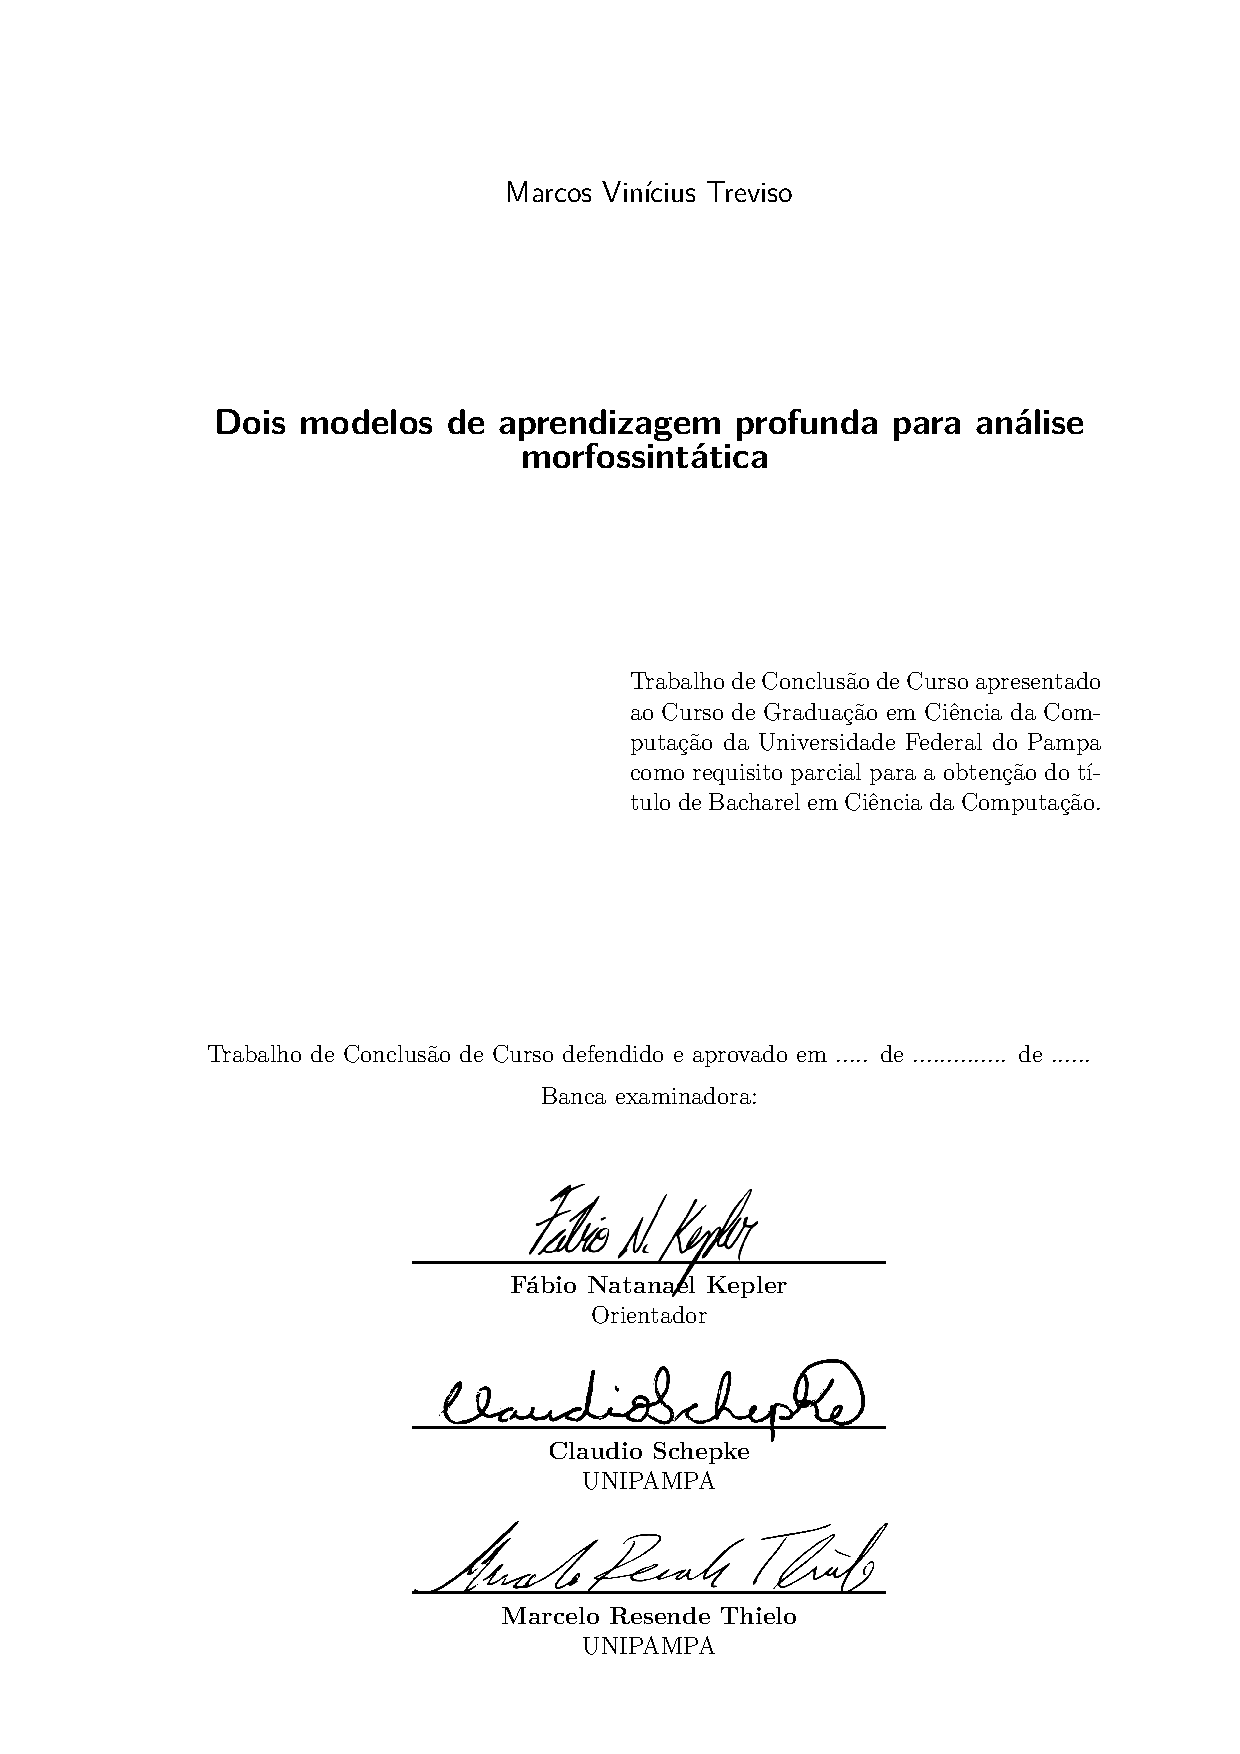
\includepdf{pretextuais/aprovacao.pdf}

% Ou, versão assinada em arquivo de imagem (jpg, png, etc)
% Mas prefira em PDF. Em imagem é preciso acertar os recuos das margens:
% \vspace*{-4cm}
% \hspace*{-3.5cm}
% 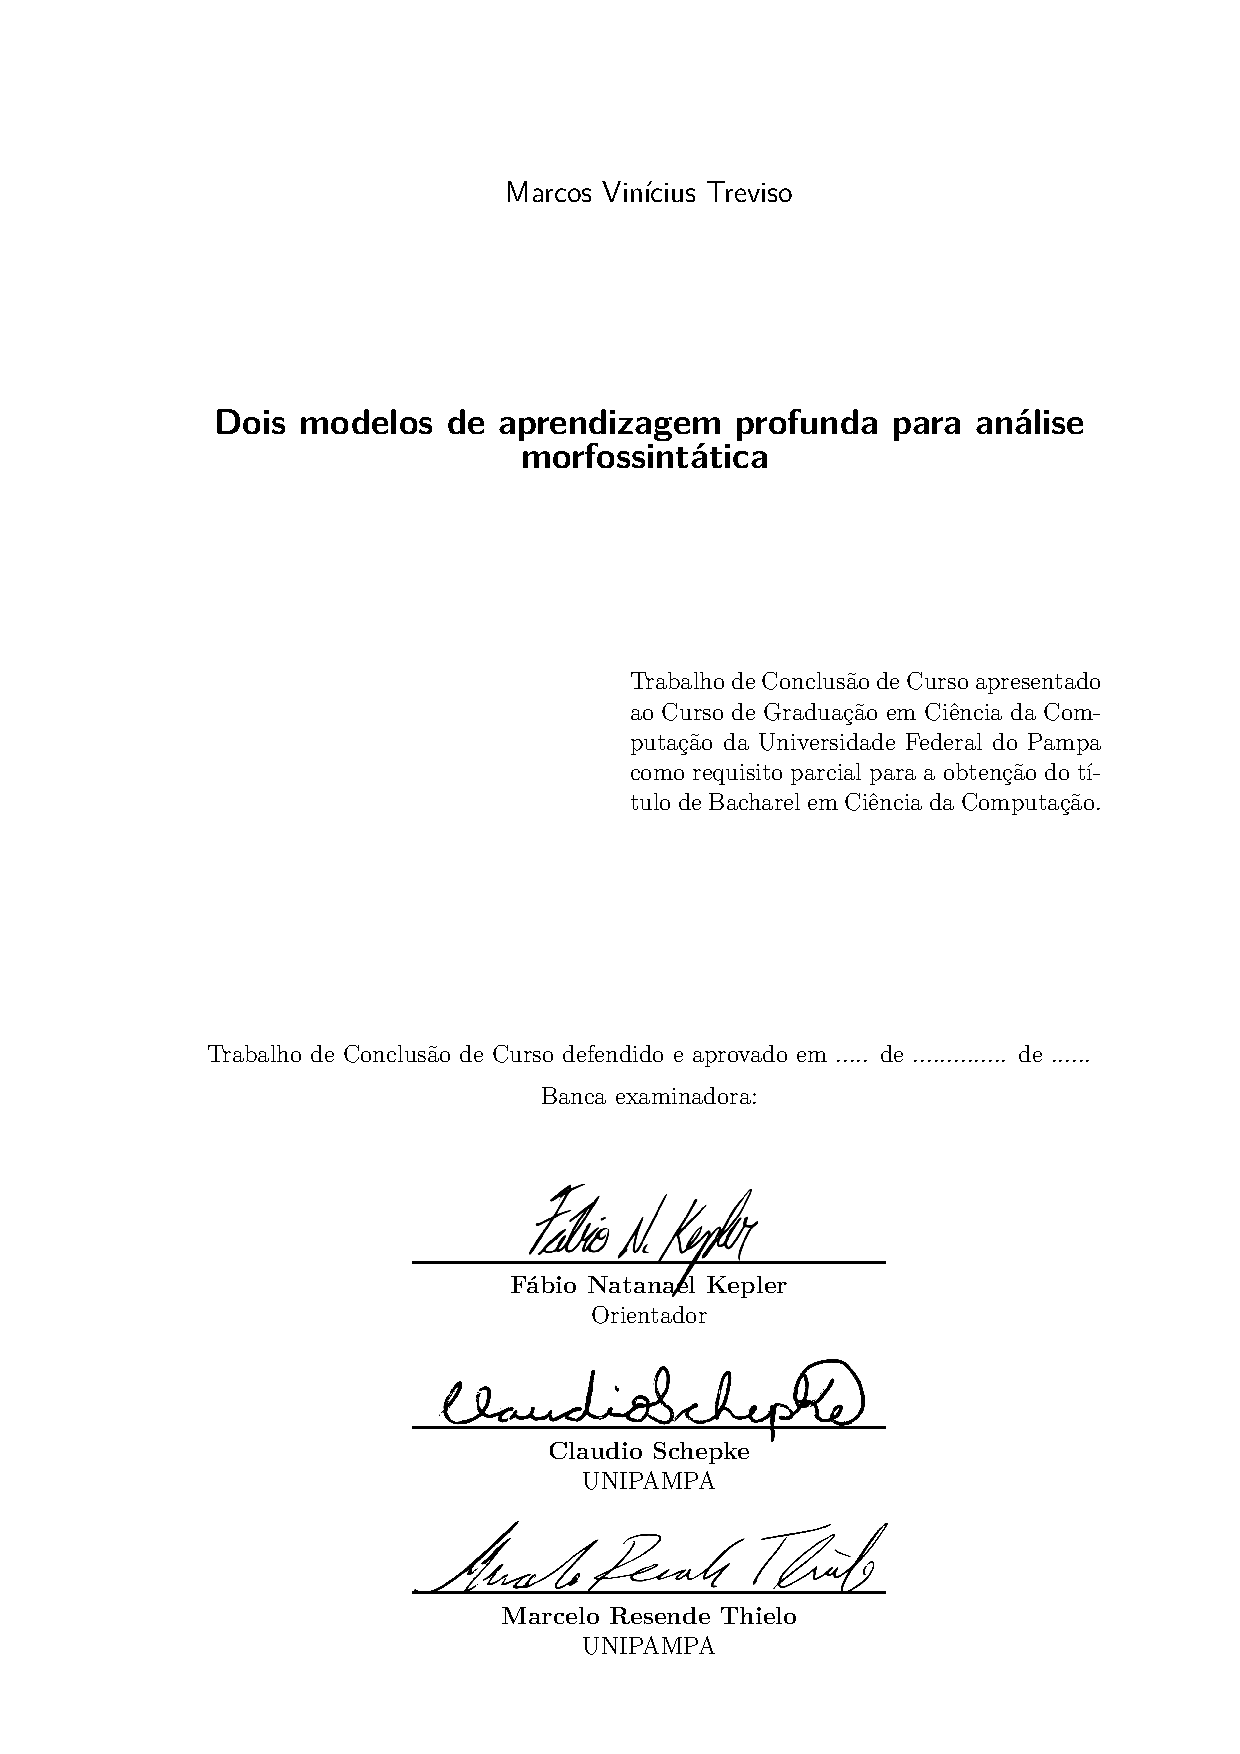
\includegraphics[width=\paperwidth]{pretextuais/aprovacao} 

\end{folhadeaprovacao}
% \end{comment}

% -----------------------------------------------
% Dedicatória [OPCIONAL]
% -----------------------------------------------
\begin{dedicatoria}
   \vspace*{\fill}
   \centering
   \noindent
   \textit{Este trabalho é dedicado às crianças adultas que,\\
   quando pequenas, sonharam em se tornar cientistas.} \vspace*{\fill}
\end{dedicatoria}

% -----------------------------------------------
% Agradecimentos [OPCIONAL]
% -----------------------------------------------
\begin{agradecimentos}


O esforço para chegar até aqui é grande, e certamente não conseguiria ter feito isso sozinho, por isso gostaria de agradecer meu orientador Fábio por me ajudar em assuntos variados durante a faculdade, com o qual aprendi muito. 

Não é só de estudo que concluímos uma faculdade, depende muito da nossa força de vontade, e nesse quesito gostaria de agradecer muito a minha irmã Thaís, e especialmente meu pai Gilmar e minha mãe Loeiri por todos os conselhos e apoio. 

Lorem ipsum dolor sit amet, consectetur adipisicing elit, sed do eiusmod
tempor incididunt ut labore et dolore magna aliqua. Ut enim ad minim veniam,
quis nostrud exercitation ullamco laboris nisi ut aliquip ex ea commodo
consequat. 

Duis aute irure dolor in reprehenderit in voluptate velit esse
cillum dolore eu fugiat nulla pariatur. Excepteur sint occaecat cupidatat non
proident, sunt in culpa qui officia deserunt mollit anim id est laborum.

\end{agradecimentos}

% -----------------------------------------------
% Epígrafe [OPCIONAL]
% -----------------------------------------------
\begin{epigrafe}
    \vspace*{\fill}
	\begin{flushright}
		\textit{"Existem muitas hipóteses em ciência que estão erradas. Isso é \\
		perfeitamente aceitável, eles são a abertura para achar as que estão certas." \\
		(Carl Sagan - O Mundo Assombrado Pelos Demônios)}
	\end{flushright}
\end{epigrafe}


% -----------------------------------------------
% Resumo [OBRIGATÓRIO]
% -----------------------------------------------
\begin{resumo}
 
Part-of-speech Tagging consiste em classificar uma palavra pertencente a um conjunto de textos em uma classe gramatical através da análise morfossintática. Apesar de muitos métodos já terem sidos propostos para essa tarefa, em Processamento de Linguagem Natural estamos sempre buscando ganhar mais performance, já que Part-of-speech Tagging pode ser aplicada em uma grande variedade de aplicações. Nós estudamos diferentes métodos para gerar representações de palavras \textit{word embeddings} a partir de uma coleção de textos denominadas córpus. Criamos então um modelo baseado em aprendizagem profunda utilizando redes neurais que recebe essas representações como entrada e gerá como saída uma classe gramatical associada. O modelo neural é guiado, onde palavras mais fáceis de serem analisadas são aplicadas primeiro na rede. Sua saída é complementada na entrada da própria palavra classificada. O treinamento é feito sobre três diferente córpus etiquetados para o português brasileiro.

 \vspace{\onelineskip}
    
 \noindent
 \textbf{Palavras-chave}: Aprendizado de máquina. Aprendizagem profunda. Processamento de linguagem natural. Part-of-speech tagging. Redes neurais. Word embeddings.
\end{resumo}


% -----------------------------------------------
% Abstract (resumo em inglês) [OBRIGATÓRIO]
% -----------------------------------------------
\begin{resumo}[Abstract]
 
Part-of-speech Tagging consists in classify a given word, that belongs to a collections of texts, with particular part of speech tag, based in its context. Despite much methods already been proposed to this task, in Natural Language Processing we are always looking for improvement, because Part-of-speech Tagging can be used in many applications. We study different methods to generate words representations (word embeddings) from a collection of texts denominated corpora. We create a deep learning model by using a recurrent neural network that receives as input the word embeddings and predicts a part-of-speech tag to the associated word. The neural model is guided, where easy words to classify are applied first in the network. The output is a vector tag, that is then complemented with the input of the same word classified. The training process occur over three different tagged corpora for brazilian portuguese.

 \vspace{\onelineskip}
 
 \noindent 
 \textbf{Key-words}: Machine learning. Deep learning. Natural language processing. Part-of-speech tagging. Neural networks. Word embeddings.
\end{resumo}


% Resumo estendido [OPCIONAL]
% \input{pretextuais/resumoest}

% -----------------------------------------------
% Listas
% -----------------------------------------------
% Figuras/Ilustrações [OPCIONAL]
\pdfbookmark[0]{\listfigurename}{lof}
\listoffigures*
\cleardoublepage
% -----------------------------------------------
% Tabelas [OPCIONAL]
\pdfbookmark[0]{\listtablename}{lot}
\listoftables*
\cleardoublepage
% -----------------------------------------------
% Abreviaturas [OPCIONAL] (veja o pacote acro e os exemplo acima)
\newcommand{\lobname}{Lista de abreviaturas}
\pdfbookmark[0]{\lobname}{lob}
\printacronyms[include-classes=abreviaturas,name=\lobname,header=chapter*]
\cleardoublepage
% -----------------------------------------------
% Siglas [OPCIONAL] (veja o pacote acro e os exemplo acima)
\newcommand{\loaname}{Lista de siglas}
\pdfbookmark[0]{\loaname}{loa}
\printacronyms[include-classes=acronimos,name=\loaname,header=chapter*]
\cleardoublepage
% -----------------------------------------------
% Símbolos [OPCIONAL] (veja o pacote nomencl e os exemplo acima)
\renewcommand{\nomname}{Lista de símbolos}
\pdfbookmark[0]{\nomname}{los}
\printnomenclature
\cleardoublepage


% -----------------------------------------------
% Sumário
% -----------------------------------------------
\pdfbookmark[0]{\contentsname}{toc}
\tableofcontents*
\cleardoublepage
% -----------------------------------------------

\begin{comment}
  %cutter={M1234x}, % INFORMAÇÃO QUE VAI NA FICHA CATALOGRÁFICA
  %cdu={100.0*01.10},  % Define o identificador CDU do documento, fornecido pela Secretaria do Curso (verificar se é necessário).
  keywords={Modelo de texto, UNIPAMPA, Latex}, % Define as palavras-chave que deverão constar na Ficha Catalográfica, separadas por vírgulas.
  firstcommitteemember={Nome membro da banca 1\\ UNIPAMPA},
  secondcommitteemember={Nome membro da banca 2\\ Instituição},
\end{comment}



% +++++++++++++++++++++++++++++++++++++++++++++++++++++++++++++++++++++++++++++++++++++++++++++++++
% ELEMENTOS TEXTUAIS
% +++++++++++++++++++++++++++++++++++++++++++++++++++++++++++++++++++++++++++++++++++++++++++++++++
% É possível usar \textual ou \mainmatter, que é a macro padrão do memoir.
\textual

% Você pode dividir o seu texto em vários arquivos. Por exemplo, um para cada seção principal do
% trabalho: introducao.tex, relacionados.tex, metodologia.tex, experimentos.tex, conclusao.tex.
%==============================================================================
\chapter{Introdução}\label{introducao}
%==============================================================================

O ato de classificar uma palavra pertencente a um conjunto de textos em uma classe gramatical depende de sua estrutura morfo-sintática, esse ato é conhecido no campo de \ac{pln} como \ac{pos} Tagging. A \autoref{fig:exemploclassificacao} ilustra esse processo. 

O conjunto de textos denominados \textit{córpus} são amplamente utilizados para esse processo, e é sobre eles que é feito o treinamento do modelo de reconhecimento de padrões para que seja possível classificar uma palavra a uma certa classe gramatical.

Um dos problemas dessa classificação é justamente a eficiência com o qual cada classe gramatical é atribuída para certa palavra, nesse quesito, há vários métodos já idealizados que conseguiram uma eficiência de cerca de 97\% \cite{dos2014training, collobert2011deep, fonseca2015evaluating}. \citeonline{fonseca2015evaluating} afirmam ter conseguido o estado-da-arte atual para o português com 97,57\% de acurácia.

Apesar de muitos desses métodos já serem utilizados em larga escala, em \ac{pln} estamos sempre buscando ganhar mais performance, já que \ac{pos} Tagging pode ser aplicada em uma grande variedade de aplicações como tradução automática e extração de informações de textos \cite{manning1999foundations}, ferramentas de auxílio à leitura e escrita \cite{marquiafavel2010processo}, entre outras.

\begin{figure}[htb]
  \caption{Exemplo de classificação gramatical}\label{fig:exemploclassificacao}
  \begin{center}
      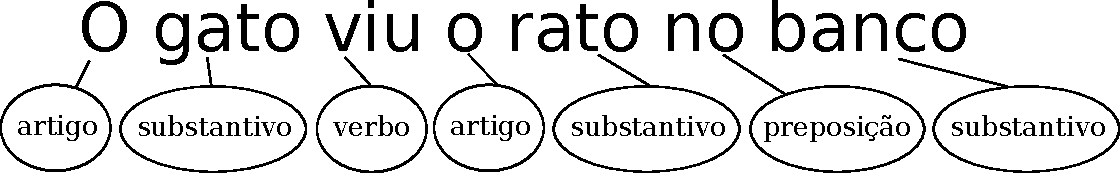
\includegraphics[scale=0.75]{img/exemploclassificacao.pdf}
  \end{center}
\end{figure}

Nosso trabalho consiste em classificar palavras de acordo com seu contexto, ou seja, é feita a análise em termos das unidades primitivas que a compõem, e uma vez que ela é cumprida, podemos aplicar o resultado em outras análises.


%------------------------------------------------------------------------------
\section{Objetivo}\label{sec:objetivo}
%------------------------------------------------------------------------------

Este trabalho tem, por fim, propor um novo método de classificação de palavras em classes gramáticais e analisar sua eficiência em relação a trabalhos já publicados que utilizam métodos já consolidados. Primordialmente, isso será feito para o escopo da língua portuguesa brasileira. 

Para buscar uma boa eficiência será proposto um método original, que se baseia em classificar primeiramente palavras mais fáceis (\textit{e.g verbos}), desse modo, espera-se deixar palavras ambíguas por último. Por exemplo, para a \autoref{fig:exemploclassificacao} deixaríamos a palavra \textit{canto} para o final, uma vez que não sabemos se isso se trata de um verbo ou de um substantivo.  

Como já mencionado, o estado-da-arte atual tem atualmente cerca de 97\% de acurácia, tentaremos ultrapassar esse limite aplicando novas técnicas de classificação e utilizando características significantes das palavras. A acurácia da classificação não será a única medida levada em consideração, o tempo de processamento gasto no treinamento para cada \textit{córpus} também será.

Para exemplificar brevemente uma possível aplicação, no final pretende-se que o modelo seja capaz de classificar corretamente as palavras analisando o seu contexto, e com isso outros analisadores conseguirão identificar o uso das palavras de acordo com seu significado, como mostrado abaixo na \autoref{eq:exemploobjetivo}. Essa equação será explicada na \autoref{sec:representacaodaspalavras}.

\begin{equation}
\texttt{homem + coroa = rei} \label{eq:exemploobjetivo}
\end{equation}



%------------------------------------------------------------------------------
\section{Estrutura do trabalho}\label{sec:estruturadotrabalho}
%------------------------------------------------------------------------------

A fim de proporcionar uma boa interpretação, este trabalho foi dividido nos seguintes capítulos: No \autoref{oproblema} será descrito o problema de etiquetagem. No \autoref{fundamentos} será mostrados os principais fundamentos necessários para entender o método proposto e seus conceitos relacionados; após passar os fundamentos, será apresentado no \autoref{trabalhosrelacionados} os trabalhos relacionados que procuram resolver o problema de \ac{pos} Tagging utilizando diferentes técnicas e abordagens. Depois, no \autoref{desenvolvimento} será detalhado aspectos da metodologia a ser aplicada e a explicação do método proposto juntamente com as técnicas utilizadas. Então, no \autoref{comparativo} será feito um comparativo entre os resultados preliminares alcançados e uma breve discussão a respeito. E por fim, no \autoref{conclusao} será apresentado as considerações finais.
 % [OBRIGATORIO]
%\part{Revisão de Literatura} % Pode-se usar partes para organizar os capítulos
%==============================================================================
\chapter{O problema}\label{oproblema}
%==============================================================================

O problema a ser resolvido não é trivial, pois linguagens naturais tem bastante ambiguidade, onde uma palavra pode possuir diferentes categorias gramaticais. Além disso, há muita ambiguidade no português do Brasil, visto que é uma língua com uma sintaxe flexível e que possui uma rica morfologia. Essa ambiguidade dificulta a análise morfossintática, porque não é possível determinar a priori qual classe gramatical a palavra sendo analisada pertence. No exemplo anterior, da \autoref{fig:exemploclassificacao}, não fica claro qual é o tipo de \textit{banco} que está sendo referenciado, onde pode ser um verbo ou um substantivo (\textit{o ato de bancar na primeira pessoa do singular do presente; um subtantivo que se refere a um local onde armazena-se dinheiro; ou um substantivo que se refere um objeto para sentar.}). Para resolver o problema da ambiguidade, é necessário analisar os lexemas vizinhos de uma dada palavra, ou seja, é preciso analisar o seu contexto associado, por exemplo:


\begin{center}
\texttt{"O rio da cidade."}
\end{center}

A palavra \textit{rio} pode ser classificada como substantivo ou como verbo, mas levando em consideração o contexto, fica evidente que a classificação correta é substantivo.

Uma estratégia trivial seria utilizar um dicionário com uma função de mapeamento de um para um, onde a \textit{chave} seria a palavra e o \textit{valor} seria a classe gramatical. Infelizmente essa técnica requer muitos recursos computacionais, visto que o número de entradas seria estupendamente grande por ter todas as palavras possíveis de português, caso contrário, haveria o
problema de ter uma palavra fora do vocabulário, e portanto ela não teria uma classe gramatical associada. Porém, o principal revés dessa estratégia é a ambiguidade, que faz com que uma palavra tenha mais que uma classe gramatical associada, e portanto não é possível mapear com indubitabilidade de que a classe associada é a correta sem antes analisar o contexto.

Dito isso, este trabalho consiste em desenvolver um método para classificar palavras em suas respectivas classes gramaticais de modo eficiente. Uma abordagem que está sendo amplamente utilizada para resolver esse problema é aprendizado de máquina, pois ela permite treinar um modelo que aprenda a classificar as palavras de acordo com o contexto em que está associada. 

E em ordem de conseguir solucionar esse problema com eficiência, é necessário escolher um bom método computacional. Este trabalho se baseará na utilização de um método de aprendizagem profunda, que utiliza modelos neurais com múltiplas camadas (\textit{deep-learning}), para que seja possível treinar modelos capazes de realizar a classificação. Utilizamos redes neurais pois elas oferecem um jeito alternativo de realizar aprendizado de máquina quando temos hipóteses complexas com muitas características diferentes. 

 % [OBRIGATORIO]

%==============================================================================
\chapter{Fundamentos}\label{fundamentos}
%==============================================================================

Devido aos impasses demonstrados no \autoref{oproblema}, este trabalho é baseado em conceitos de aprendizado de máquina, que dedica-se na elaboraçãode algoritmos e técnicas que permitem um computador a aprender padrões.  

\section{Aprendizado de máquina}\label{sec:aprendizadodemaquina}

Para realizar a aprendizagem é necessário, a princípio, dados de entrada que servem como exemplo para nosso modelo, com esses dados é possível treinar o modelo para que ele possa então aprender com base nesses exemplos. Depois de realizar o treinamento, é possível generalizar sobre outros dados ainda não testados e gerar uma resposta apropriada como saída. O diagrama da \autoref{fig:passoapasso} abaixo mostra os passos para obter o resultado final.

\begin{figure}[htb]
	  \caption{Diagrama para resultado final}\label{fig:passoapasso}
	  \begin{center}
	      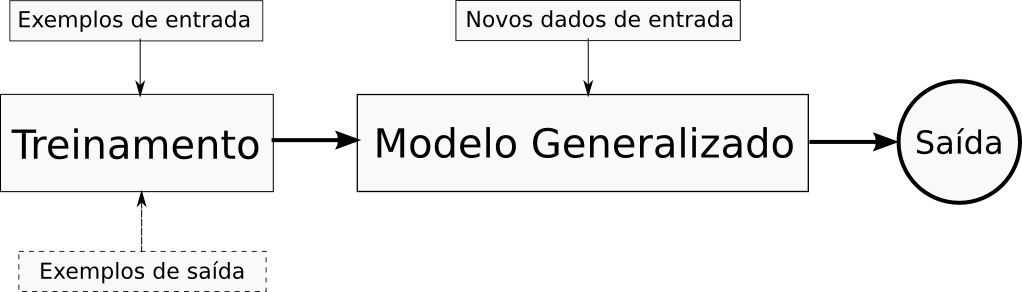
\includegraphics[scale=0.5]{img/passoapasso}
	  \end{center}
\end{figure}


O aprendizado de máquina pode ser dividido em duas abordagens: O \textbf{aprendizado supervisionado}, onde é dado um conjunto de dados de entrada e já se sabe como a saída deve parecer, tendo a ideia de que há uma relação entre a entrada e a saída; O \textbf{aprendizado não supervisionado}, que nos permite abordar problemas com pouca ou até nenhuma ideia de como os resultados devem parecer, nesse caso a caixa de exemplos de saída pode não existir.

Neste trabalho a abordagem utilizada vai ser o aprendizado supervisionado, pois já temos uma classe gramatical apropriada para cada palavra em seu contexto.

O aprendizado supervisionado permite dividir os problemas em duas categorias distintas:


\begin{itemize}
	\item \textbf{Regressão}: Tenta-se prever resultados com uma saída contínua, significando que deseja-se mapear variáveis de entrada em alguma função contínua. A \autoref{fig:demregressao} demonstra esse processo. Nessa demonstração, os círculos em vermelho são dados de exemplo, já a reta azul representa a predição feita pela regressão.
	\item \textbf{Classificação}:  Tenta-se prever resultados em uma saída discreta, ou seja, deseja0se mapear variáveis de entrada em categoriais discretas. A \autoref{fig:demclassificacao} demonstra esse processo. Essa demonstração tem duas classes diferentes, as representadas pelos círculos amarelos e pelas cruzes vermelhas, já o contorno em verde representa o resultado da classificação sobre esses dados de exemplo.
\end{itemize}


\begin{figure}[htb]
	  \caption{Demonstração de regressão}\label{fig:demregressao}
	  \begin{center}
	      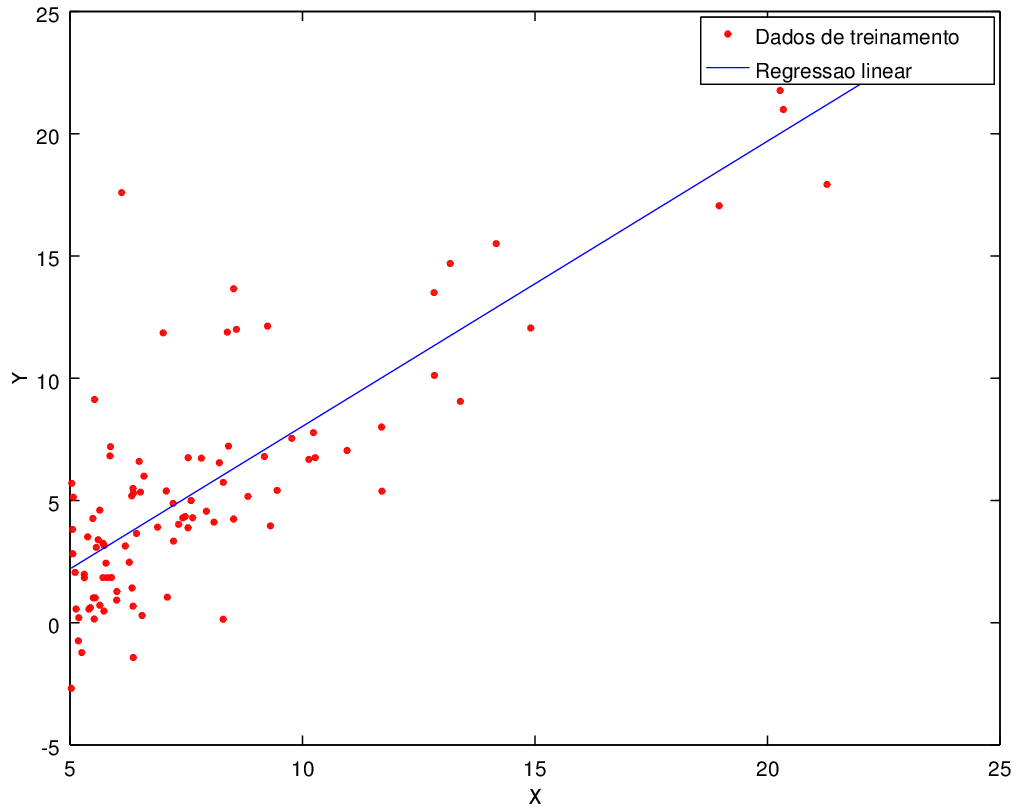
\includegraphics[scale=0.75]{img/regressao2}
	  \end{center}
	  \legend{Fonte: \citeonline{machinelearningcoursera}}
\end{figure}

\begin{figure}[htb]
  \caption{Demonstração de classificação}\label{fig:demclassificacao}
  \begin{center}
      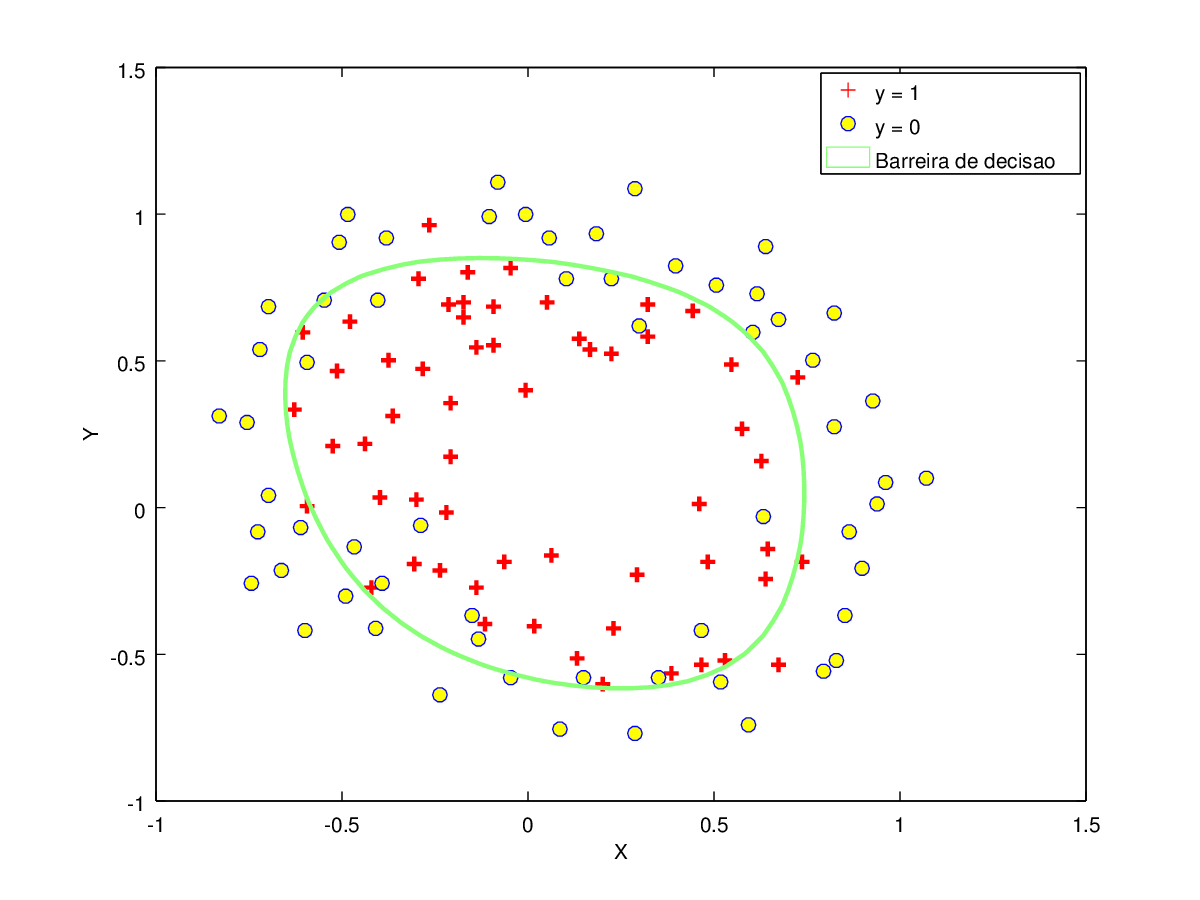
\includegraphics[scale=0.75]{img/classificacao2}
  \end{center}
  \legend{Fonte: \citeonline{machinelearningcoursera}}
\end{figure}


Logo adiante será explicado os fundamentos de classificação e uma técnica para resolver esse problema chamada de regressão logística \cite{hosmer2004applied}. E em virtude de apresentar conceitos fundamentais há serem aplicados posteriormente nas redes neurais profundas, será falado um pouco mais sobre regressão logística, e também sobre propriedades importantes que serão referenciadas durante todo o trabalho.

\subsection{Classificação}

Em um problema de classificação, nossa saída \textit{Y} vai ser um vetor com valores sendo apenas zero ou um.

\begin{equation}\label{eq:binaryclassification}
Y \in \{0, 1\}
\end{equation}

A equação \ref{eq:binaryclassification} está tratando apenas duas classes. Sendo assim, esse problema é chamado de classificação binária. Para resolver esse problema, um método que pode ser utilizado é regressão logística.

A fim de simplificar o uso das variáveis, faremos o uso de uma notação que é normalmente utilizada em textos de aprendizado de máquina, ela pode ser vista na \autoref{tab:classificacaonomenclatura}.

\begin{table}[!htb]
\caption{Nomenclaturas} \label{tab:classificacaonomenclatura}
\begin{center}
\begin{tabular}{m{2cm}m{14.0cm}}
  \toprule
  $X$ & dados de entrada ou \textit{features} \\
  $Y$ & dados de saída \\
  $X_j^{(i)}$ & o valor da \textit{feature} \textit{j} no i-ésimo exemplo de treinamento \\
  $X^{(i)}$ & o vetor coluna de todas as \textit{features} no i-ésimo exemplo de treinamento \\
  $m$ & número de exemplos de treinamento \\
  $n$ & $|X^{(i)}|$, o número de \textit{features} \\
  $(x, y)$ & um exemplo de treinamento \\
  $(X^{(i)}, Y^{(i)})$ & o i-ésimo exemplo de treinamento \\
  $\theta$ & parâmetros a serem aprendidos \\
  \bottomrule
\end{tabular}
\legend{Notação utilizada para classificação}
\end{center}

\end{table}



\ \\
\ \\

\subsection{Função de hipótese}

A função de hipótese descreve a confiança dos dados de entrada para os dados de saída, para isso é atribuido valores para os parâmetros $\theta$s. Essa relação está definida na \autoref{eq:funcaodehipotese}. Observe que ela tem apenas dois parâmetros. Na realidade uma hipótese pode ter vários parâmetros relacionados com os dados de entrada \textit{X}, se tiver \textit{n} dados de entrada, então haverá \textit{n+1} parâmetros. A forma geral da função de hipótese está mostrada na \autoref{eq:funcaodehipotesegeral}.

\begin{align}
h_{\theta}(x) = &\ \theta_0 + \theta_1 x \label{eq:funcaodehipotese} \\
h_{\theta}(x) = &\ \theta_0 + \theta_1 x_1 + \theta_2 x_2 + ... + \theta_n x_n \label{eq:funcaodehipotesegeral}
\end{align}

Uma maneira de simplificar a função de hipótese é trabalhar com a definição de multiplicação de matrizes. Então a função de hipótese pode ser representada de uma forma vetorizada, como mostrado na \autoref{eq:funcaodehipotesegeralvet}. Para maiores informações a respeito de matrizes e vetores, consultar o Anexo \ref{anexo:algebralinear}, que traz informações básicas de álgebra linear.

\begin{equation}
h_{\theta}(x) = \big[\theta_0\ \theta_1\ ...\ \theta_n\big] \times \begin{bmatrix} x_0 \\ x_1 \\ \vdots \\ x_n \end{bmatrix}  = \theta^TX \label{eq:funcaodehipotesegeralvet}
\end{equation}

Para que seja possível fazer operações de matrizes com $\theta$ e $X$, será setado $X_0^{(i)} = 1$ para todos os valores de $i$. Isso faz com que os vetores $\theta$ e $X^{(i)}$ combinem um com o outro elementarmente.

Uma função de hipótese tem o objetivo de mapear funções aleatórias dentro do intervalo de saída \textit{Y}. Portanto, nossa função de hipótese deve satisfazer a \autoref{eq:reglogicfuncaohip}.

\begin{equation}\label{eq:reglogicfuncaohip}
0 \leq h_{\theta}(x) \leq 1
\end{equation}

Para fazer com que uma entrada contínua fique nesse intervalo, é necessário utilizar uma função linear que faça esse mapeamento de modo linear, e para isso mudamos a forma da função de hipótese. A nova forma usa a função sigmoide, também conhecida como função logística.

\begin{align}
h_{\theta}(x) = g(\theta^TX) \nonumber \\
z = \theta^TX \nonumber \\
g(z) = \frac{1}{1 + e^{-z}} \label{eq:funcaosigmoide}
\end{align}

\begin{figure}[!htb]
  \caption{Função sigmoide}
  \label{fig:funcaosigmoide}
  \begin{center}
  \begin{tikzpicture}
  \begin{axis}[
  		width=.8\textwidth,
		scaled ticks=false,
		log ticks with fixed point,
		ymin=0,ymax=1,xmin=-10,xmax=10,domain=-10:10,
		log basis y = 10,
		xlabel=X,
      	ylabel=Y,
      	legend style={draw=none},
      	samples=200,
    ]
    \addplot[blue] { 1 / (1 + pow(e, -x))};
  \end{axis}
  \end{tikzpicture}
  \end{center}
\end{figure}

A função da \autoref{eq:funcaosigmoide} representada na fígura \autoref{fig:funcaosigmoide} mapeia qualquer número no intervalo [0, 1], tornando isso útil para transformar qualquer valor arbitrário em uma função mais ideal para problemas de classificação.

Para calcular a função de hipótese, podemos colocar o $\theta^TX$ na função logística. Isso nos dará a probabilidade de que a saída é 1.

\begin{equation}
h_{\theta}(x) = P(y=1 | X ; \theta) = 1 - P(y=0 | X ; \theta) \nonumber
\end{equation}

Ou seja, a probabilidade de nossa predição ser 1 é o oposto da probabilidade de ser 0. Sendo assim, a soma das probabilidades para \textit{y = 0} e \textit{y = 1} deve ser 1.

Para ter uma classificação discreta podemos traduzir a saída da função de hipótese de acordo com a \autoref{eq:decisionboundary}:
\begin{align} 
h_{\theta}(x) \geq 0.5 \Rightarrow y = 1 \nonumber \\
h_{\theta}(x) < 0.5 \Rightarrow y = 0 \label{eq:decisionboundary}
\end{align}

Então, se a entrada é $\theta^TX$, isso significa que:
\begin{equation}
h_{\theta}(x) = g(\theta^TX) \geq 0.5 \quad \text{ quando } \quad \theta^TX \geq 0 \nonumber
\end{equation}

A partir disso, podemos dizer que:
\begin{align}
\theta^TX \geq 0 \Rightarrow y = 1 \nonumber \\
\theta^TX < 0 \Rightarrow y = 0 \nonumber
\end{align}

O \textbf{limite de decisão} (ou barreira de decisão) é a linha que separa a área quando \textit{y = 0} e quando \textit{y = 1}. Isso é criado pela função de hipótese. Uma observação importante é que a função de hipótese não precisa ser linear, pode ser até mesmo um círculo ou ter qualquer forma para ajustar os dados, como mostrado na \autoref{fig:demclassificacao}. Isto é, uma função de hipótese pode ter várias \textit{features}. Novas \textit{features} podem ser criadas ao combinar as \textit{features} já existentes e modificando-as. Por exemplo, se houvesse dois dados de entrada $x_1$ e $x_2$, seria possível criar a função de hipótese:

\begin{equation}
\nonumber
h_{\theta}(x) = \theta_0 + \theta_1 x_1 + \theta_2 x_2 + \theta_3 x_1 x_2 + \theta_4 x_1^2 + \theta_5 x_2^2 + \theta_6 x_1^2 x_2^2 + \cdots
\end{equation}

Todavia, essa abordagem pode gerar problemas de desempenho. Algumas \textit{features} podem também acabar se tornando obsoletas e não ajudar em nada no resultado final, tornando seu cálculo inútil. Mas o principal problema dessa abordagem é o \textit{overfitting}, que faz com que a função de hipótese interpole os dados, esse problema será explicado na \autoref{subsec:regularizacao}.


\subsection{Função de custo}

Para medir a precisão da função de hipótese é necessário uma função que diga o quão precisa aquela hipótese é, tal função é denominada de função de custo. Com ela, é feita uma média de todos os resultados das hipóteses com a entrada \textit{X} comparada com o valor objetivo \textit{Y}. Ela pode ser expressa como na \autoref{eq:funcaodecusto}.

\begin{equation}
\label{eq:funcaodecusto}
J(\theta) = \frac{1}{m}\sum\limits_{i=1}^{m}Custo(h_{\theta}(x^{(i)}, y^{(i)}))
\end{equation}

Onde,


\begin{align}
 Custo(h_{\theta}(x^{(i)}, y^{(i)}) = \left\{
  \begin{array}{l l} 
    -log(h_{\theta}(x)) & \quad \text{se } y=1 \\
    -log(1 - h_{\theta}(x)) & \quad \text{se } y=0 \label{eq:funcaocusto}
  \end{array} \right.
\end{align}


A \autoref{eq:funcaocusto} captura a intuição de que se $h_\theta(x) = 0$, mas $y = 1$, então o algoritmo de aprendizado será penalizado por um custo muito alto. A \autoref{fig:logfunctions} demonstra os dois respectivos casos dessa equação.


\begin{figure}[!htb]
  \caption{Representação dos casos da função de custo}
  \label{fig:logfunctions}
  \begin{center}
  \begin{tikzpicture}

  % \draw[step=1cm,gray,very thin] (0,0) grid (11.3, 9.5);

  \begin{axis}[
  		width=.8\textwidth,
		scaled ticks=false,
		xlabel=$x$,
		log ticks with fixed point,
		ymin=0,ymax=2,xmin=0,xmax=1,domain=0:1,
		log basis y = 10,
      	legend style={draw=none},
      	samples=200,
    ]
    \addplot[blue] { - ln(x)/ln(10)};
    \addplot[orange] { - ln(1 - x)/ln(10)};
    \addlegendentry{$-log(h_{\theta}(x))$}
    \addlegendentry{$-log(1 - h_{\theta}(x))$}
  \end{axis}
  \end{tikzpicture}
  \end{center}
\end{figure}


O quanto mais a função de hipótese está longe de \textit{y}, maior é a saída da função de custo. Se a função de hipótese é igual a \textit{y}, então o custo é 0.

Podemos simplificar a \autoref{eq:funcaocusto} com dois casos condicionais em apenas um caso:

\begin{equation} 
\label{eq:funcaodecustosimplificada}
Custo(h_{\theta}(x), y) = -ylog(h_{\theta}(x)) - (1-y)log(1 - h_{\theta}(x))
\end{equation}

Nota-se que quando \textit{y} é igual a 1, o segundo termo será 0 e não afetará o resultado. E quando \textit{y} é igual a 0, o primeiro termo será 0 e não afetara o resultado. Aplicando a \autoref{eq:funcaodecustosimplificada} na função de custo da equação \autoref{eq:funcaodecusto}, podemos reescrê-la como a equação \autoref{eq:funcaodecustofinal} ou na versão vetorizada da \autoref{eq:funcaodecustovet}.

\begin{equation}
\label{eq:funcaodecustofinal}
J(\theta) = - \frac{1}{m}\sum\limits_{i=1}^{m}\Big( y^{(i)}log(h_{\theta}(x^{(i)})) + (1-y^{(i)})log(1 - h_{\theta}(x^{(i)})) \Big)
\end{equation}

\begin{equation}
J(\theta) = - \frac{1}{m}\Big( log(g(X\theta))^TY + log(1 - g(X\theta))^T(1 - Y) \Big) \label{eq:funcaodecustovet}
\end{equation}

O objetivo da regressão logística é minimizar a função de custo em relação aos parâmetros $\theta$s. Usando dois parâmetros é possível visualizar uma função de custo através do número de iterações, isso pode ser observado no exemplo da \autoref{fig:funcaodecustosurf} e da \autoref{fig:funcaodecustocontorno}. 


\begin{figure}
  \caption{Função de custo - $J(\theta_0, \theta_1)$}
  \begin{subfigure}[htb]{0.5\textwidth} \label{fig:funcaodecustosurf}
    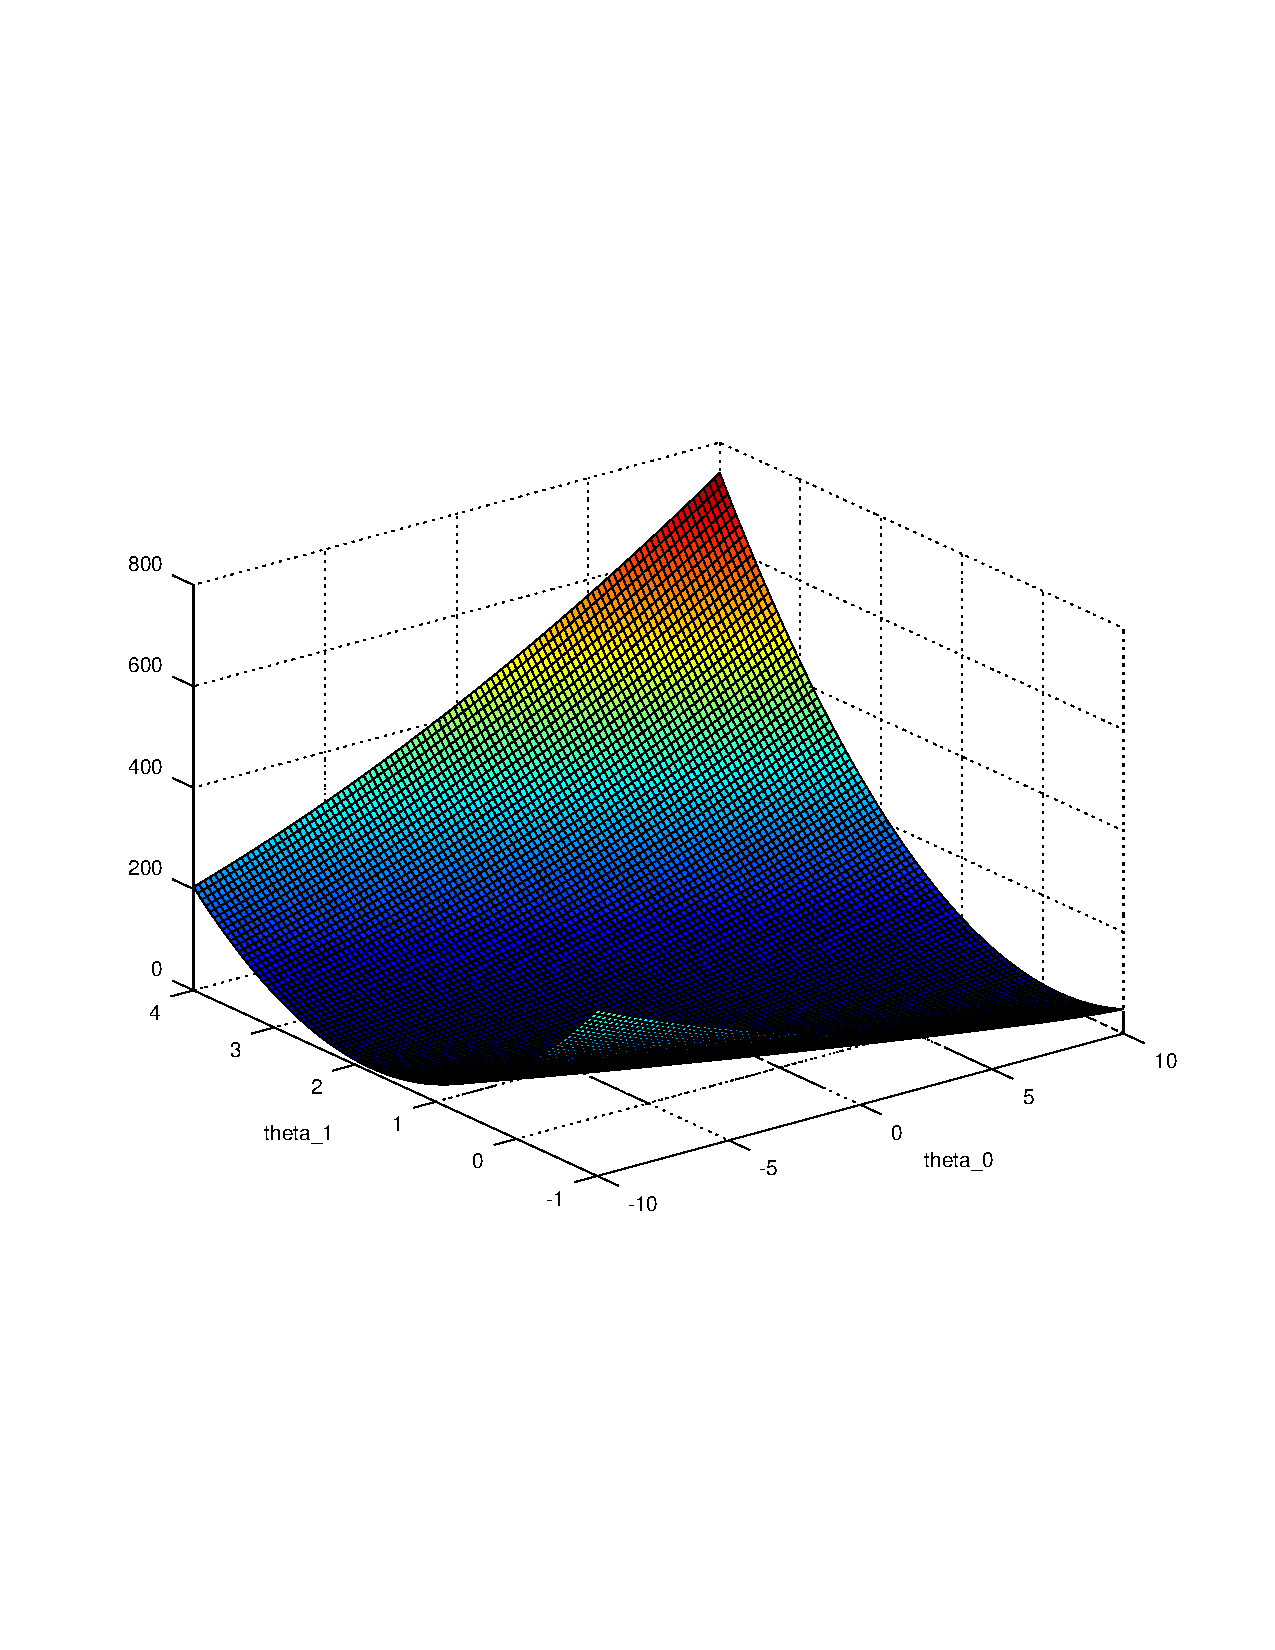
\includegraphics[width=\textwidth]{img/funcaodecustosurf} 
    \legend{(a) Gráfico de superfície} 
  \end{subfigure} 
  %
  \begin{subfigure}[htb]{0.5\textwidth} \label{fig:funcaodecustocontorno}
    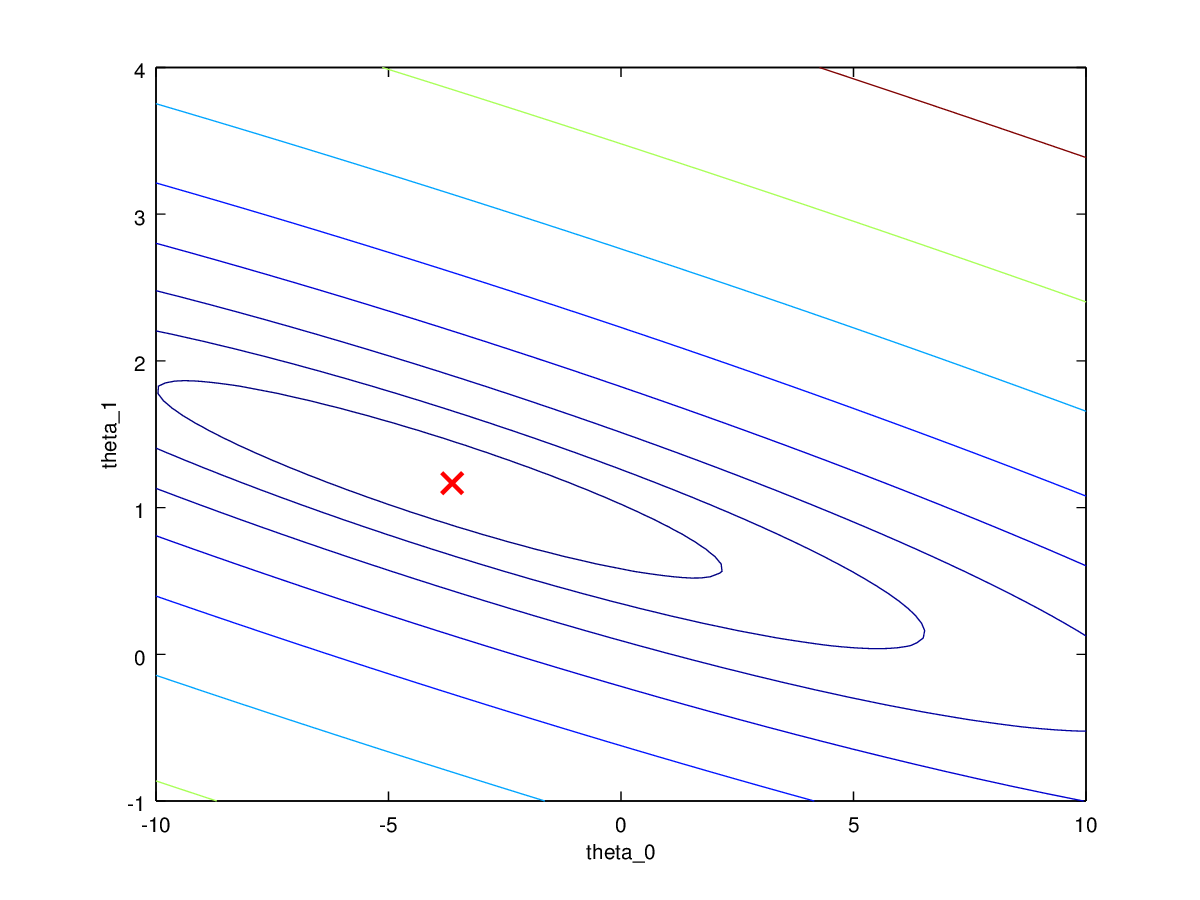
\includegraphics[width=\textwidth]{img/funcaodecustocontorno} 
    \legend{(b) Gráfico de contorno}
  \end{subfigure} 

  \legend{Fonte: \citeonline{machinelearningcoursera}}
\end{figure}


\subsection{Minimização da função de custo}

Para essa tarefa é necessário a aplicação de um algoritmo que pega a função de custo e tente minimizá-la, e por fim retorne os valores dos parâmetros $ \theta $s aprendidos. Com isso, estaremos melhorando nossa função de hipótese. 

Um dos algoritmos mais utilizados para essa tarefa é o \textbf{Gradiente Descendente} \cite{michalski2013machine}, seu funcionamento baseia-se em seguir a derivida da função de custo em relação aos parâmetros $\theta$s alternadamente, com isso a encosta da tangente dará a direção para seguir adiante. Ademais, é aplicada uma taxa de aprendizagem $ \alpha $ a cada iteração, para tentar controlar a convergência.

Seu funcionamento é descrito pelo algoritmo \ref{eq:gradientedesc}.

\textit{repita até convergir \{}
\begin{equation}
\label{eq:gradientedesc}
\quad \theta_j := \theta_j = \alpha \frac{\partial}{\partial\theta_j} J(\theta)
\end{equation}
\textit{\quad\quad\quad \}}

Ao trabalhar sobre a derivada parcial da função de custo, podemos chegar na \autoref{eq:gradientefinal} e adiante na versão vetorizada na \autoref{eq:gradientefinalvet}. A explicação de como trabalhar sobre a derivada pode ser encontrado no \autoref{app:derivadasgraddesc}.

\begin{equation}
\quad \theta_j := \theta_j = \alpha \sum\limits_{i=1}^{m}\Big(h_{\theta}(x^{(i)}) - y^{(i)} \Big) x_j^{(i)} \label{eq:gradientefinal}
\end{equation}

\begin{equation}
\quad \theta := \theta - \frac{\alpha}{m}X^T(g(X\theta) - Y) \label{eq:gradientefinalvet}
\end{equation}

Na \autoref{fig:funcgraddesc} é possível visualizar esse funcionamento sobre os parâmetros. Observe que nesse caso o algoritmo consegue convergir para o mínimo global, porém em alguns casos (dependendo de nossa taxa de aprendizagem $ \alpha $) pode-se convergir para um mínimo local como mostrado na \autoref{fig:funcgraddescnot}. Basicamente se $\alpha$ for um valor muito alto, os passos para o mínimal ótimo serão grandes e portanto o risco de divergência é maior, caso seja muito baixo, os passos para o mínimal ótimo serão pequenos e portanto vai demorar muito para convergir. Em \cite{machinelearningcoursera}, é dito para testar manualmente esse valor, começando com 0,001 e subindo multiplicando por 10 esse valor até atingir uma divergência no resultado. Sendo assim possível analisar o melhor valor da taxa de aprendizagem e selecioná-la para o treinamento definitivo.

\begin{figure}
  \caption{Funcionamento do Gradiente Descendente}
  \begin{subfigure}[htb]{0.5\textwidth} \label{fig:funcgraddesc}
    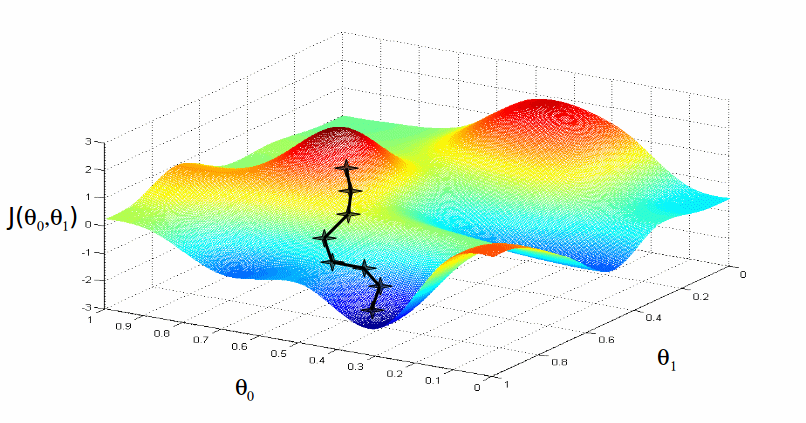
\includegraphics[width=\textwidth]{img/funcgraddesc1}
    \legend{(a) Convergindo para uma mínimo global} 
  \end{subfigure}
  %
  \begin{subfigure}[htb]{0.5\textwidth} \label{fig:funcgraddescnot}
    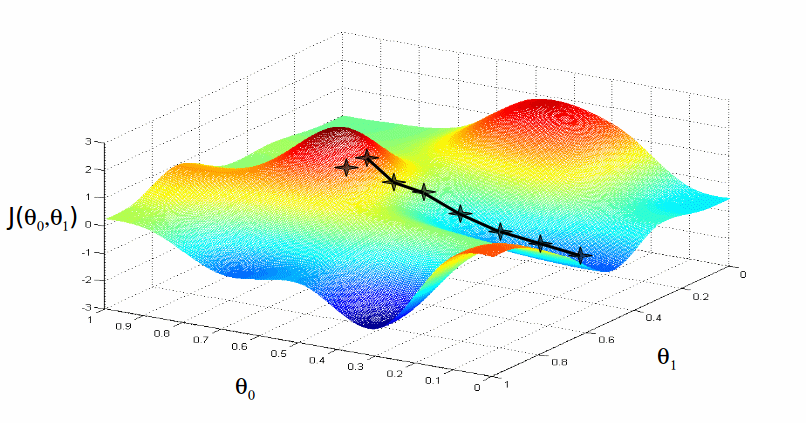
\includegraphics[width=\textwidth]{img/funcgraddesc2}
    \legend{(b) Convergindo para uma mínimo local}
  \end{subfigure}

  \legend{Fonte: \citeonline{machinelearningcoursera}}
\end{figure}

O Gradiente Descendente é apenas um dos vários algoritmos que existem para minimizar a função de custo. De acordo com \cite{machinelearningcoursera}, há alternativas mais sofisticadas como o Gradiente Conjugado, BFGS e L-BFGS, onde além de serem mais rápidos que o Gradiente Descendente, eles não precisam selecionar manualmente o valor de $\alpha$. Mas, também é sugerido que não devemos tentar codificar esses algoritmos, visto que são mais complexos e requerem um bom conhecimento de cálculo numérico.


\subsection{Classificação multiclasse}

O \ac{pos} Tagging é um problema de classificação multiclasse, onde deve-se etiquetar uma palavra em uma de várias categorias gramaticais possíveis. É possível fazer isso ao expandir nossa definição para que a saída seja $y = \{0, 1, ..., n\}$. Nesse caso, é dividido o problema em \textit{n + 1} problemas de classificação binária e em cada um será feito a predizagem da probabilidade de que $y$ é membro de uma dessas classes.
\begin{align}
h_{\theta}^{(0)}(X) =&  P(y=0 | X ; \theta) \nonumber \\
h_{\theta}^{(1)}(X) =&  P(y=1 | X ; \theta) \nonumber \\
\vdots & \nonumber \\
h_{\theta}^{(n)}(X) =&  P(y=n | X ; \theta) \nonumber
\end{align}

E então escolhe-se a classe com o valor de hipótese mais alto.
\begin{equation}
prediction = max_i(h_{\theta}^{(i)}(X)) \nonumber
\end{equation}


\subsection{Regularização}\label{subsec:regularizacao}

Como já mencionado, regularização é um conceito importante designado para resolver o problema de \textit{overfitting}.

Quando se trabalha com abordagens de aprendizagem supervisionada, tem dois problemas que podem ocorrer dependendo das \textit{features} escolhidas. O \textbf{\textit{underfitting}} ocorre quando a forma da função de hipótese mapeia mal à tendência dos dados. Isso é causado por uma função que é muito simples ou que usa pouquíssimas \textit{features}. Em contrapartida, \textbf{\textit{overfitting}} é causado por uma função de hipótese que encaixa os dados avaliados mas não generaliza bem para classificar novos dados. É usualmente causado por uma função complexa que cria muitas curvas e ângulos desnecessários não relacionados aos dados.

\begin{figure}
  
  \caption{Exemplo de \textit{underfitting} e \textit{overfitting}} \label{fig:exemplounderover}
  
  \begin{subfigure}[htb]{0.5\textwidth}
    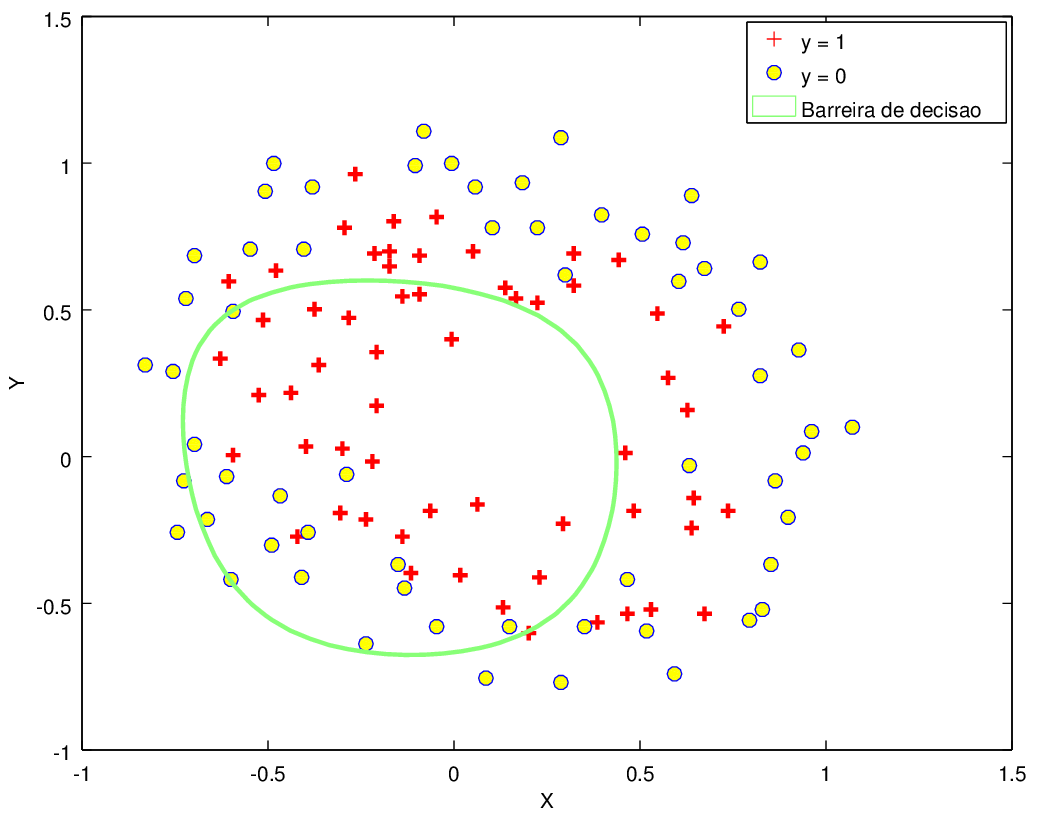
\includegraphics[width=\textwidth]{img/underfittingex}
    \legend{(a) \textit{underfitting}} 
  \end{subfigure}
  %
  \begin{subfigure}[htb]{0.5\textwidth}
    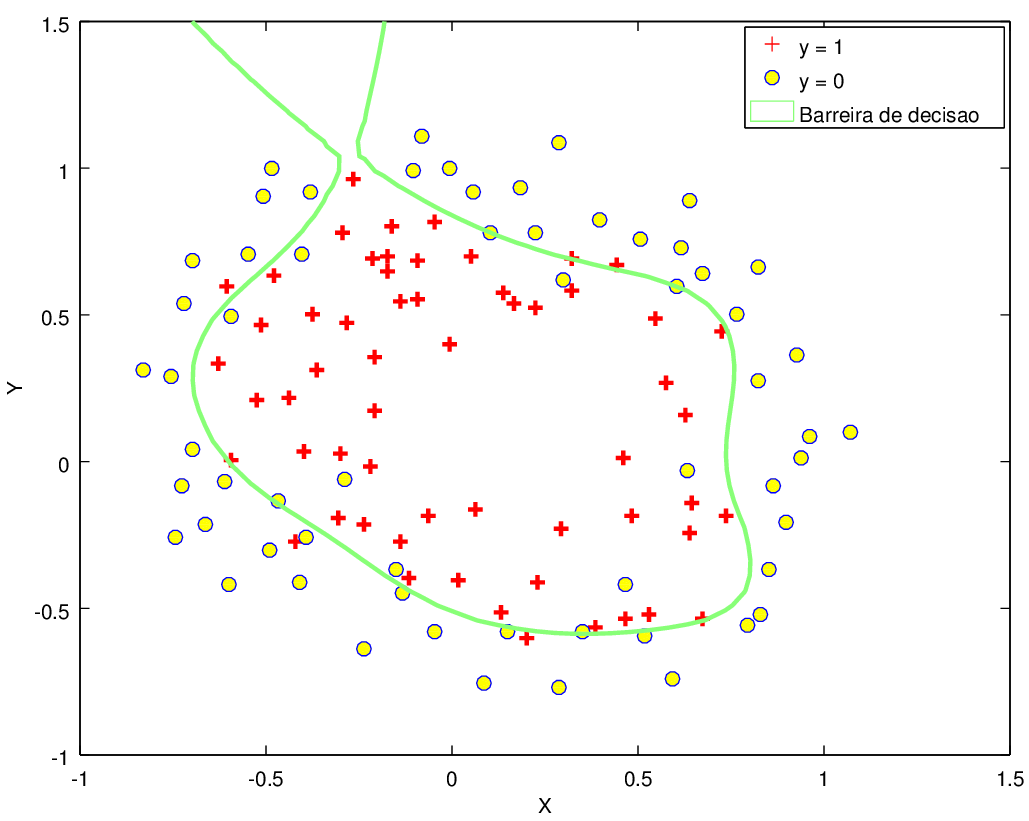
\includegraphics[width=\textwidth]{img/overfittingex}
    \legend{(b) \textit{overfitting}}
  \end{subfigure}

  \legend{Fonte: \citeonline{machinelearningcoursera}}
\end{figure}

A classificação ideal para o conjunto de dados mostrados na \autoref{fig:exemplounderover} é o exemplo mostrado na \autoref{fig:demclassificacao}.

Segundo \cite{machinelearningcoursera}, há duas opções principais para resolver o problema de \textit{overfitting}:

\begin{alineas}
	\item Reduzir o número de \textit{features}:
		\begin{alineas}
			\item Manualmente selecionar quais \textit{features} usar;
			\item Usar um algoritmo de seleção de modelo.
		\end{alineas}
	\item Regularização:
		\begin{alineas}
			\item Manter todos as \textit{features}, mas reduzir os parâmetros $\theta_j$.
		\end{alineas}
\end{alineas}

Em geral, regularização funciona bem quando há bastante features levemente úteis.


\section{Córpus e seu conjunto de classes gramaticais}

Córpus são uma coleção de textos colocados como um só, eles são os exemplos de entrada para nosso treinamento. A qualidade e o tamanho desses córpus são importantes para que o etiquetador possa generalizar sentenças ainda não vistas. Eles contém também um conjunto de classes gramaticais associadas a cada palavra.

Esses conjuntos podem se diferenciar na sua granularidade, como por exemplo, podem ter diferentes classes gramaticais para nomes no plural e no singular, ou agrupar eles em uma única classe \cite{fonseca2015evaluating}. No inglês, há vários conjunto de classes gramaticais de qualidade que são amplamento utilizados, são o Penn Treebank tagset \cite{penntreebank}, CLAWS5 e CLAWS7.

Já no português, os córpus estão evoluindo com o tempo, embora alguns erros são encontrados neles \cite{fonseca2013mac}, eles ainda são a melhor opção devido a seu tamanho e qualidade, os principais e mais utilizados para essa tarefa são o Mac-Morpho \cite{aluisio2003account} com cerca de um milhão de palavras, que retrata artigos publicados na Folha de São Paulo em 1994. O Tycho Brahe \cite{temponi2004corpus} que também tem cerca de um milhão de palavras e retrata assuntos históricos de 66 textos diferentes. Temos também o Bosque \cite{afonso2002floresta}, que contém cerca de 185 mil palavras. Além desses, \cite{fonseca2015evaluating} apresenta uma versão revisada do Mac-Morpho, com classes gramaticais novas e junção de outras. 

Infelizmente esses córpus não podem ser combinados em um só, já que eles se diferenciam no conjunto de classes gramaticais e também no seu uso associado. Uma possível alternativa para essa combinação, seria o uso de uma aprendizagem não supervisionada, aplicando técnicas de clusterização.

A aprendizagem baseada em córpus tem se mostrado uma estratégia atrativa, já que pode ser usado recursos criados com melhores performance [X, Y, Z]. Devido a isso, nesse trabalho vamos utilizar três córpus: o Mac-Morpho original; Mac-Morpho revisado e o Tycho Brahe. O conjunto de etiquetas para esses córpus podem ser encontrados, respectivamente, em \cite{aluisio2003account}, \cite{fonseca2015evaluating} e \cite{temponi2004corpus}.



\section{Representação das palavras}\label{sec:representacaodaspalavras}

Palavras \footnote{Uma palavra pode ser qualquer conjunto de caracteres, inclusive pontuações, números, etc.} podem ser representadas de várias maneiras em um modelo de aprendizagem, podendo ser até mesmo feito o uso real da palavra como um conjunto de caracteres.

No entanto, a melhor abordagem e a mais indicada atualmente é a utilização de \textit{word embeddings}, elas são representação de palavras como vetores reais valorados em um espaço multidimensional \cite{turian2010word}. Elas podem ser geradas de maneiras diferentes dependendo da técnica utilizada, clássicas abordagens baseiam-se na frequência e co-ocorrência das palavras, até mesmo via modelos de redes neurais \cite{dos2014training}. Um dos processos de criação é mostrado na \autoref{fig:criacaowordemb}.

\begin{figure}[htb]
  \caption{Exemplo de criação de \textit{word embeddings}} \label{fig:criacaowordemb}
  \begin{center}
      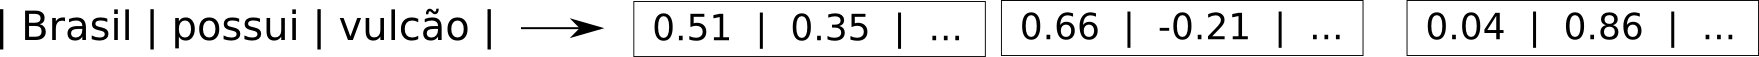
\includegraphics[scale=0.3]{img/criacaowordemb}
  \end{center}
\end{figure}


Ou seja, dada uma palavra \textit{word}, temos a transformação \textit{W}:
\begin{equation}
W:word \to \mathbb{R}^n
\end{equation}

Em ordem de prever esses valores com precisão, a rede precisa aprender bons parâmetros para \textit{W}.

A grande vantagem em se utilizar \textit{word embeddings} é o fato dessa técnica conseguir capturar informações sintáticas e semânticas das palavras. Isso pode ser visualizado através do t-SNE \cite{van2008visualizing}, uma técnica sofisticada para visualizar dados em altas dimensões.

\begin{figure}[htb]
  \caption{t-SNE: Visualização para \textit{word embeddings}}\label{fig:wordtsne}
  \begin{center}
      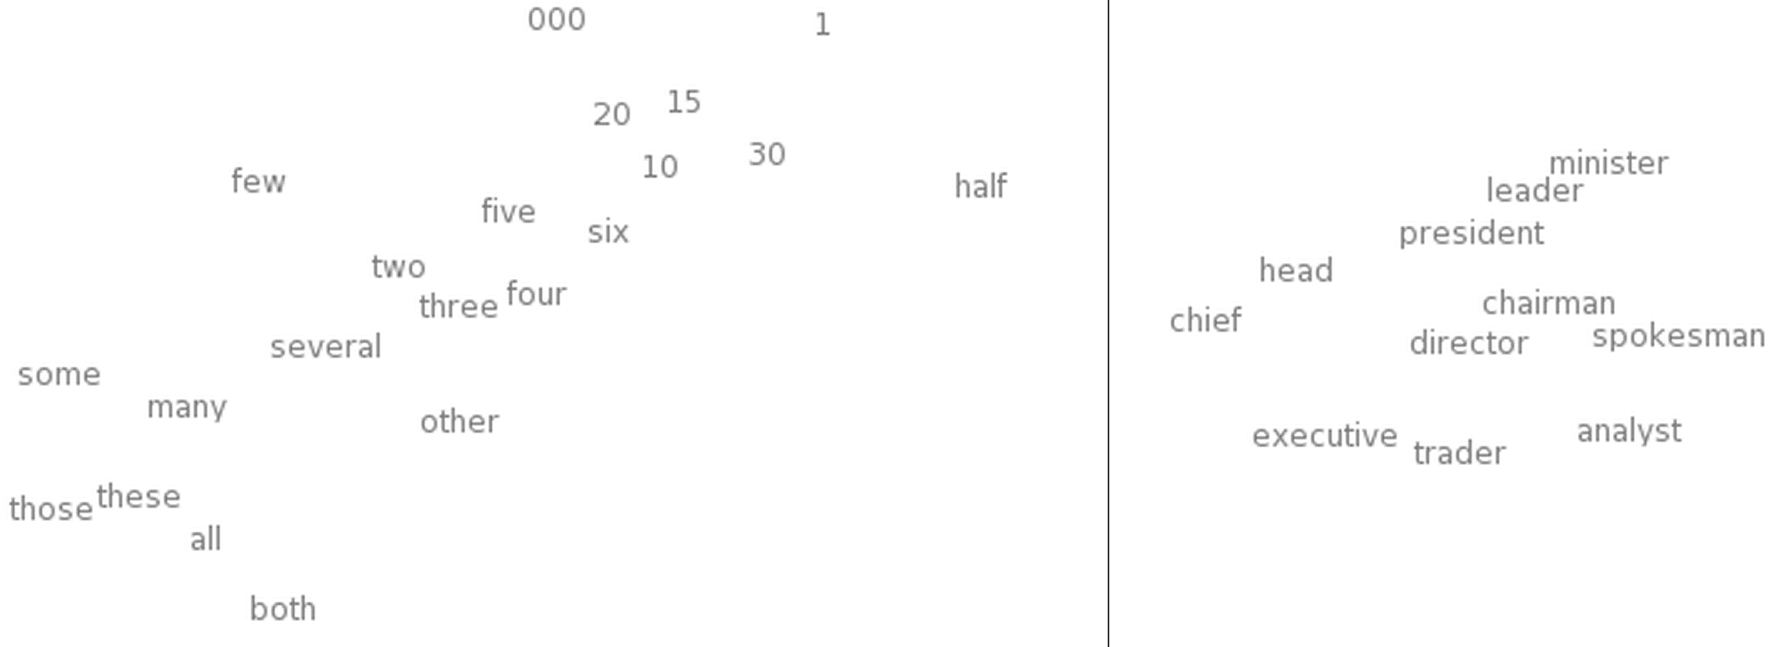
\includegraphics[scale=0.25]{img/Turian-WordTSNE}
  \end{center}
  \legend{Fonte: \citeonline{turian2010word}}
\end{figure}

Na \autoref{fig:wordtsne} podemos visualizar um tipo de mapeamento entre os sentidos intuitivos das palavras, onde na esquerda estão palavras referentes a números e na direita palavras referentes a profissões. Ou seja, palavras similares estão pertos umas das outras.

\begin{figure}[htb]
  \caption{Exemplo de palavras similares}\label{fig:palavrassimilares}
  \begin{center}
      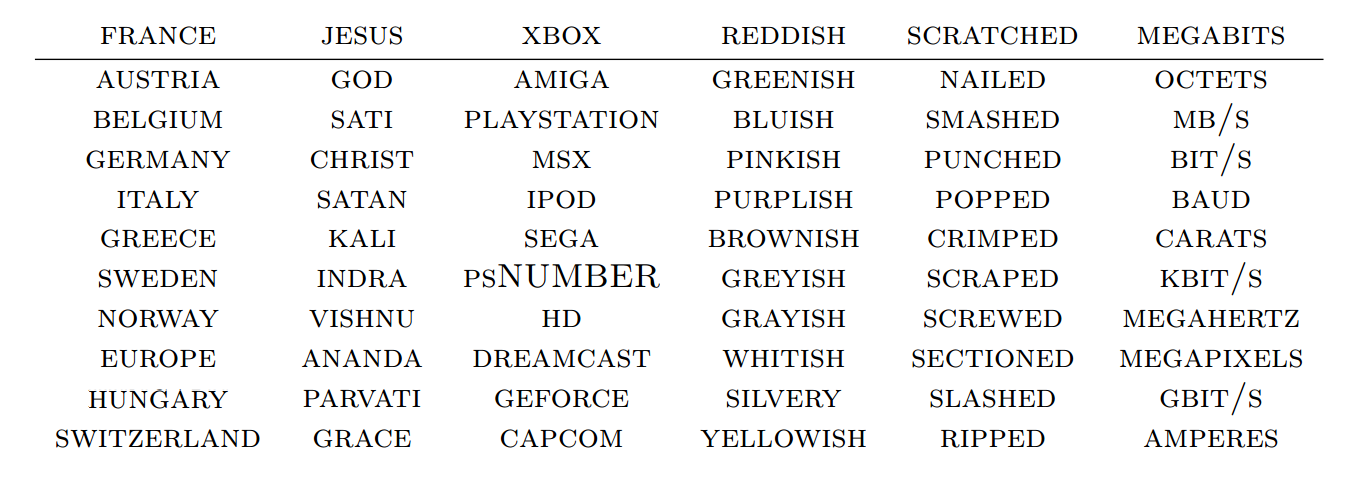
\includegraphics[scale=0.25]{img/Colbert-WordTable2}
  \end{center}
  \legend{Fonte: \citeonline{collobert2011natural}}
\end{figure}

Na \autoref{fig:palavrassimilares} temos mais alguns exemplos desse conceito, com isso podemos realizar tarefas semânticas mais facilmente, como o exemplo \ref{eq:exemploobjetivo}, que é o que esperamos obter.

Para mais informações sobre \textit{word embeddings} consultar [X] e [Y].



\section{Redes neurais}

O que escrever aqui? 

- Conceitos basicos de redes neurais



\section{Aprendizagem profunda}

- Redes neurais profundas e seus algoritmos % [OBRIGATORIO]

%==============================================================================
\chapter{Trabalhos relacionados}\label{trabalhosrelacionados}
%==============================================================================

Vários métodos já foram propostos para resolver esse mesmo problema em português brasileiro, apesar de nenhum deles ter um aproveitamento de 100\%, vários conseguiram ótimos resultados e utilizaram variadas técnicas para isso.

É apresentado em \cite{kepler2005etiquetador} um etiquetador morfossintático baseado em cadeias de Markov. É realizado testes com dois etiquetadores diferentes, um baseado em Cadeias de Markov Ocultas (HMM, do inglês \textit{Hidden Markov Models}), e outro baseado em Cadeias de Markov de Tamanho variável (VLMC, do inglês \textit{Variable Length Markov Chains}). A representação das palavras é feita de forma simples, pois a etiquetagem baseia-se em modelos probabilísticos, onde a etiqueta de uma palavra depende da própria palavra e de etiquetas anteriores. Ele é testado sobre o \textit{córpus} Tycho Brahe, e apresenta uma precisão de 95,51\% com o etiquetador VLMC, essa precisão é alcançada com um tempo de aprendizagem + etiquetagem de 157 segundos. 

Em \cite{dos2014training} é apresentado um etiquetador que aprende automaticamente as features a serem usadas através de uma rede neural profunda, que emprega uma camada evolutiva capaz de aprender \textit{embeddings} em nível de caractere e em nível de palavra. Essa rede neural profunda é conhecida como CharWNN e foi proposta originalmente por \citeonline{collobert2011natural}. Além disso, é usado um modelo em janela utilizado em \cite{collobert2011natural} para atribuir classes gramaticais para cada palavra em uma sentença. Essa estratégia assume que a classe de uma palavra depende geralmente das palavras vizinhas. No fim é utilizado o algoritmo de Viterbi \cite{viterbi1967error} para prever qual a sequência de classes gramaticais é a mais provável para aquela sentença. Esse trabalho usa três diferentes \textit{córpus} para o treinamento: o Mac-Morpho original; o Mac-Morpho (versão 2) revisado em \cite{fonseca2013mac}; e o Tycho Brahe. Eles avaliam seu modelo sobre palavras fora do vocabulário e sobre palavras presentes no vocabulário. Com o Mac-Morpho foi obtido o melhor desempenho do trabalho, uma acurácia de 97,47\%. Nesse trabalho não é mostrado estatísticas de tempo de treinamento e etiquetagem.

O mais recente etiquetador para o português brasileiro é mostrado em \cite{fonseca2015evaluating}, onde é utilizado diferentes técnicas de representação das palavras: vetores gerados de forma aleatória, \ac{nlm}, \ac{hal}, \ac{sg}. É feita então uma comparação entre elas. Nele é implementado um modelo de rede neural idealizado em \cite{collobert2008unified}, que se baseia em uma rede neural simples com múltiplas camadas, que recebe as \textit{word embeggins} como entrada e aprende a sua classe gramatical. Para isso, eles realizam o treinamento utilizando o Tycho Brahe, a versão original do Mac-Morpho (versão 1), a revisada pelos mesmos autores em um trabalho anterior \cite{fonseca2013mac} (versão 2), e também sobre mais uma versão do Mac-Morpho (versão 3) revisado por eles nesse mesmo trabalho. Atualmente, \citeonline{fonseca2015evaluating} dizem ter alcançado o estado da arte do \ac{pos} Tagging para o português brasileiro, com uma acurácia de 97,57\% sobre o Mac-Morpho original utilizando \ac{nlm} como representação das palavras. Esse trabalho não apresenta estatísticas de tempo de treinamento e etiquetagem.

A \autoref{tab:comparacaotrabsrel} sumarizada as técnicas encontradas pelos trabalhos relacionados. Já a \autoref{tab:comparacaotrabsrelac} mostra os melhores resultados para cada \textit{córpus}.

\begin{table}[!htb]
\footnotesize
\centering
\caption{Comparativo das técnicas encontradas na literatura para POS Tagging}
\label{tab:comparacaotrabsrel}
\begin{tabular}{m{3cm}m{2.5cm}m{4.1cm}m{5cm}}
  \toprule
  \textbf{Autores} & \textbf{Modelo}  & \textbf{Representação das palavras}  & \textbf{Córpus} \\
  \midrule
  \citeonline{kepler2005etiquetador} & VLMM & Sequência de caracteres & Tycho Brahe \\
  \citeonline{dos2014training} & Redes neurais profundas  & Vetores (CharWNN) & Tycho Brahe; Mac-Morpho (versões 1, 2) \\
  \citeonline{fonseca2015evaluating} & Redes neurais & Vetores (\ac{nlm}, \ac{hal}, \ac{sg}) & Tycho Brahe; Mac-Morpho (versões 1, 2, 3) \\
  Este trabalho & Redes neurais recursivas & Vetores (\ac{nlm}, \ac{sg}, \ac{glove}) & Tycho Brahe; Mac-Morpho (versões 1, 3) \\
  \bottomrule
\end{tabular}
\end{table}

\begin{table}[!htb]
\footnotesize
\centering
\caption{Comparativo dos melhores resultados encontrados na literatura para POS Tagging}
\label{tab:comparacaotrabsrelac}
\begin{tabular}{llP{3cm}P{3cm}}
  \toprule
  \textbf{Autores} & \textbf{Córpus} & \textbf{Acurácia (Todas Palavras)} & \textbf{Acurácia (\ac{fdv})} \\
  \midrule
  \centering
  \citeonline{kepler2005etiquetador} & Tycho Brahe & 95,51\% & 69,53\% \\
  \citeonline{dos2014training} 		 & Tycho Brahe & 97,17\% & 86,63\% \\
  \citeonline{dos2014training} 		 & Mac-Morpho versão 1 & 97,47\% & 89,74\% \\
  \citeonline{dos2014training} 		 & Mac-Morpho versão 2 & 97,31\% & 92,61\% \\
  \citeonline{fonseca2015evaluating} \tablefootnote{\label{notenlm} Usando \ac{nlm} como representação das palavras.} & Tycho Brahe & 96,91\% & 84,14\% \\
  \citeonline{fonseca2015evaluating} \footnoteref{notenlm} & Mac-Morpho versão 1 & 97,57\% & 93,38\% \\
  \citeonline{fonseca2015evaluating} \footnoteref{notenlm} & Mac-Morpho versão 2 & 97,48\% & 94,34\% \\
  \citeonline{fonseca2015evaluating} \footnoteref{notenlm} & Mac-Morpho versão 3 & 97,33\% & 93,66\% \\
  \bottomrule
\end{tabular}
\end{table}


% nome trab - modelo - representacao  - corpus - acuracia - tempo % [OBRIGATORIO]

%==============================================================================
\chapter{Metodologia}\label{desenvolvimento}
%==============================================================================

Neste capítulo será explicado o método proposto para resolver o problema de \ac{pos} Tagging, onde primeiramente será definida as técnicas utilizadas para seu funcionamento.

Com a intuição de simplificar o entendimento, já definimos variáveis que serão utilizadas no método de aprendizagem. Elas podem ser encontradas na \autoref{tab:variaveisdesenvolvimento}.

\begin{table}[!htb]
\caption{Notação utilizada para o treinamento do modelo} \label{tab:variaveisdesenvolvimento}
\begin{center}
\begin{tabular}{m{2cm}m{12.0cm}}
  \toprule
  $d$		& dimensão das palavras vetorizadas \\
  $t$		& tamanho da janela de palavras \\
  $\omega$	& conjunto de palavras \\
  $\gamma$  & conjunto de classes gramaticais \\
  $c_i^t$  & sequência de classes gramaticais que começa em $i$ e termina em $t$ \\
  $w_i^t$  & sequência de palavras que começa em $i$ e termina em $t$ \\
  $c_i$		& i-ésima classe gramatical \\
  $z_i$		& i-ésima classe vetorizada com dimensão $d$ \\ 
  $w_i$		& i-ésima palavra\\
  $v_i$		& i-ésima palavra vetorizada com dimensão $d$ \\
  $V_i$		& vetor centrado em $i$ com as $t$ palavras vetorizadas concatenadas \\
  $s_c(V_i)$ & pontuação de uma sequência $V_i$ ter a classe gramatical $c$ \\
  $A_{c,d,e}$ & pontuação de ir de uma classe $c$, passar por $d$ e chegar a $e$ \\
  $Q$	&	conjunto com os índices das palavras vetorizadas já classificadas \\
  \bottomrule
\end{tabular}
\end{center}

\end{table}



\section{Representação das palavras}

Seguimos a ideia explorada em massa pela literatura de representar as palavras através de vetores reais com uma dimensão fixa $d$ definida pelo usuário. Isso será feito utilizando três estratégias já mencionadas: \ac{nlm}, \ac{sg} e \ac{glove}. Ou seja, para cada $w_i \in \omega$, geramos o vetor $v_i \in \mathbb{R}^d $.

Além das \textit{word embeddings}, utilizaremos outras duas \textit{features} importantes no contexto de \ac{pos} Tagging, como capitalização que consegue, na maioria das vezes, distinguir nomeações, e também prefixos, que podem ser usadas para distinguir medidas de tempo, velocidade, etc. 

Em ordem de manter a rede neural homogênea, também iremos transformar cada classe gramatical em um vetor. Com isso poderemos aplicar funções que combinam características do vetor de uma palavra com o vetor de uma classe gramatical.


\section{Pontuações para estrutura gramatical}

Para classificar palavras em uma sentença, o etiquetador obtém uma janela de palavras de tamanho fixo a cada momento, e transforma as palavras em vetores de \textit{features}, que são então passadas para uma rede neural descrita em \cite{collobert2008unified}. A rede atribui para cada classe gramatical $c \in \gamma$ uma pontuação. A etapa de gerar pontuações para a palavra ocorre no mesmo momento que o treinamento do modelo. A saída para toda a sentença é então passada para o algoritmo de Viterbi \cite{viterbi1967error}, que realiza uma predição estruturada em um tempo polinomial.

Seguimos a estratégia apresentada em \cite{dos2014training} para realizar as pontuações. Nela, a ideia é de que a classe gramatical de uma palavra depende fortemente das palavras vizinhas, o que é verdade para várias aplicações de \ac{pln}, incluindo \ac{pos} Tagging.

Dada uma janela com $t$ palavras $\{w_1, w_2, ..., w_t\}$, que foram transformadas para sua representação vetorial $\{v_1, v_2, ..., v_t\}$, para computar a n-ésima palavra, é centralizada a janela em $n$ e concatena-se todas as palavras da metade à esquerda e da metade à direita em um novo vetor $V_n$ de dimensão $t * d$. Para palavras no começo ou no fim da sentença, é usado vetores com valores fixos para preencher o espaço vazio na janela de palavras. A \autoref{eq:janeladevets} demonstra isso.

\begin{equation} \label{eq:janeladevets}
V_n = \big\{ v_{n - (t-1)/2}, ..., v_n, ..., v_{{n + (t-1)/2}} \big\}
\end{equation}

Seguimos \cite{fonseca2015evaluating} e computamos a pontuação $s_c(V_n)$ para cada classe gramatical $c$ da palavra no meio da janela. 


Além disso, usamos a ideia apresentada em \cite{collobert2011natural}, onde é feito um esquema de predição que leva em consideração a estrutura gramatical. O método usa uma pontuação de transição $A_{c,d}$, inicializada com 0, para ir de uma classe $c \in \gamma$ para uma classe $d \in \gamma$ conforme a sequência das palavras. Porém extendemos a notação para funcionar com trigramas: $A_{c,d,e}$. A estrutura $A$ consegue armazenar informações importantes como ``após um pronome é bastante provável que há um verbo''. Depois que a rede produz a pontuação para todas as palavras, a pontuação final de uma sequência de classes gramaticais $c_1^t$ para uma sequência de palavras $w_1^t$, é dada pela \autoref{eq:pontuacaofinal}. $Q$ representa um conjunto com os índices das palavras que já foram classificadas.

\begin{equation} \label{eq:pontuacaofinal}
S(w_1^t, c_1^t) = \sum\limits_{k=1}^{t} \Big( \argmax_{1 \leq i \leq t, v_i \notin Q} (s_{c_i}(V_i) + A_{c_{i-1}, c_{i}, c_{i+1}}) \Big)
\end{equation}

Após computar isso para cada palavra na sentença, a classe gramatical final é prevista através do algoritmo de Viterbi.


\section{Treinamento}

Realizamos um treinamento supervisionado utilizando uma rede neural recursiva para a classificação das palavras em suas respectivas classes gramaticais. O modelo completo da rede neural pode ser visto na \autoref{fig:neuralnetworkfinal}.

\begin{figure}[htb]
    \caption{Modelo da rede neural}\label{fig:neuralnetworkfinal}
    \begin{center}
        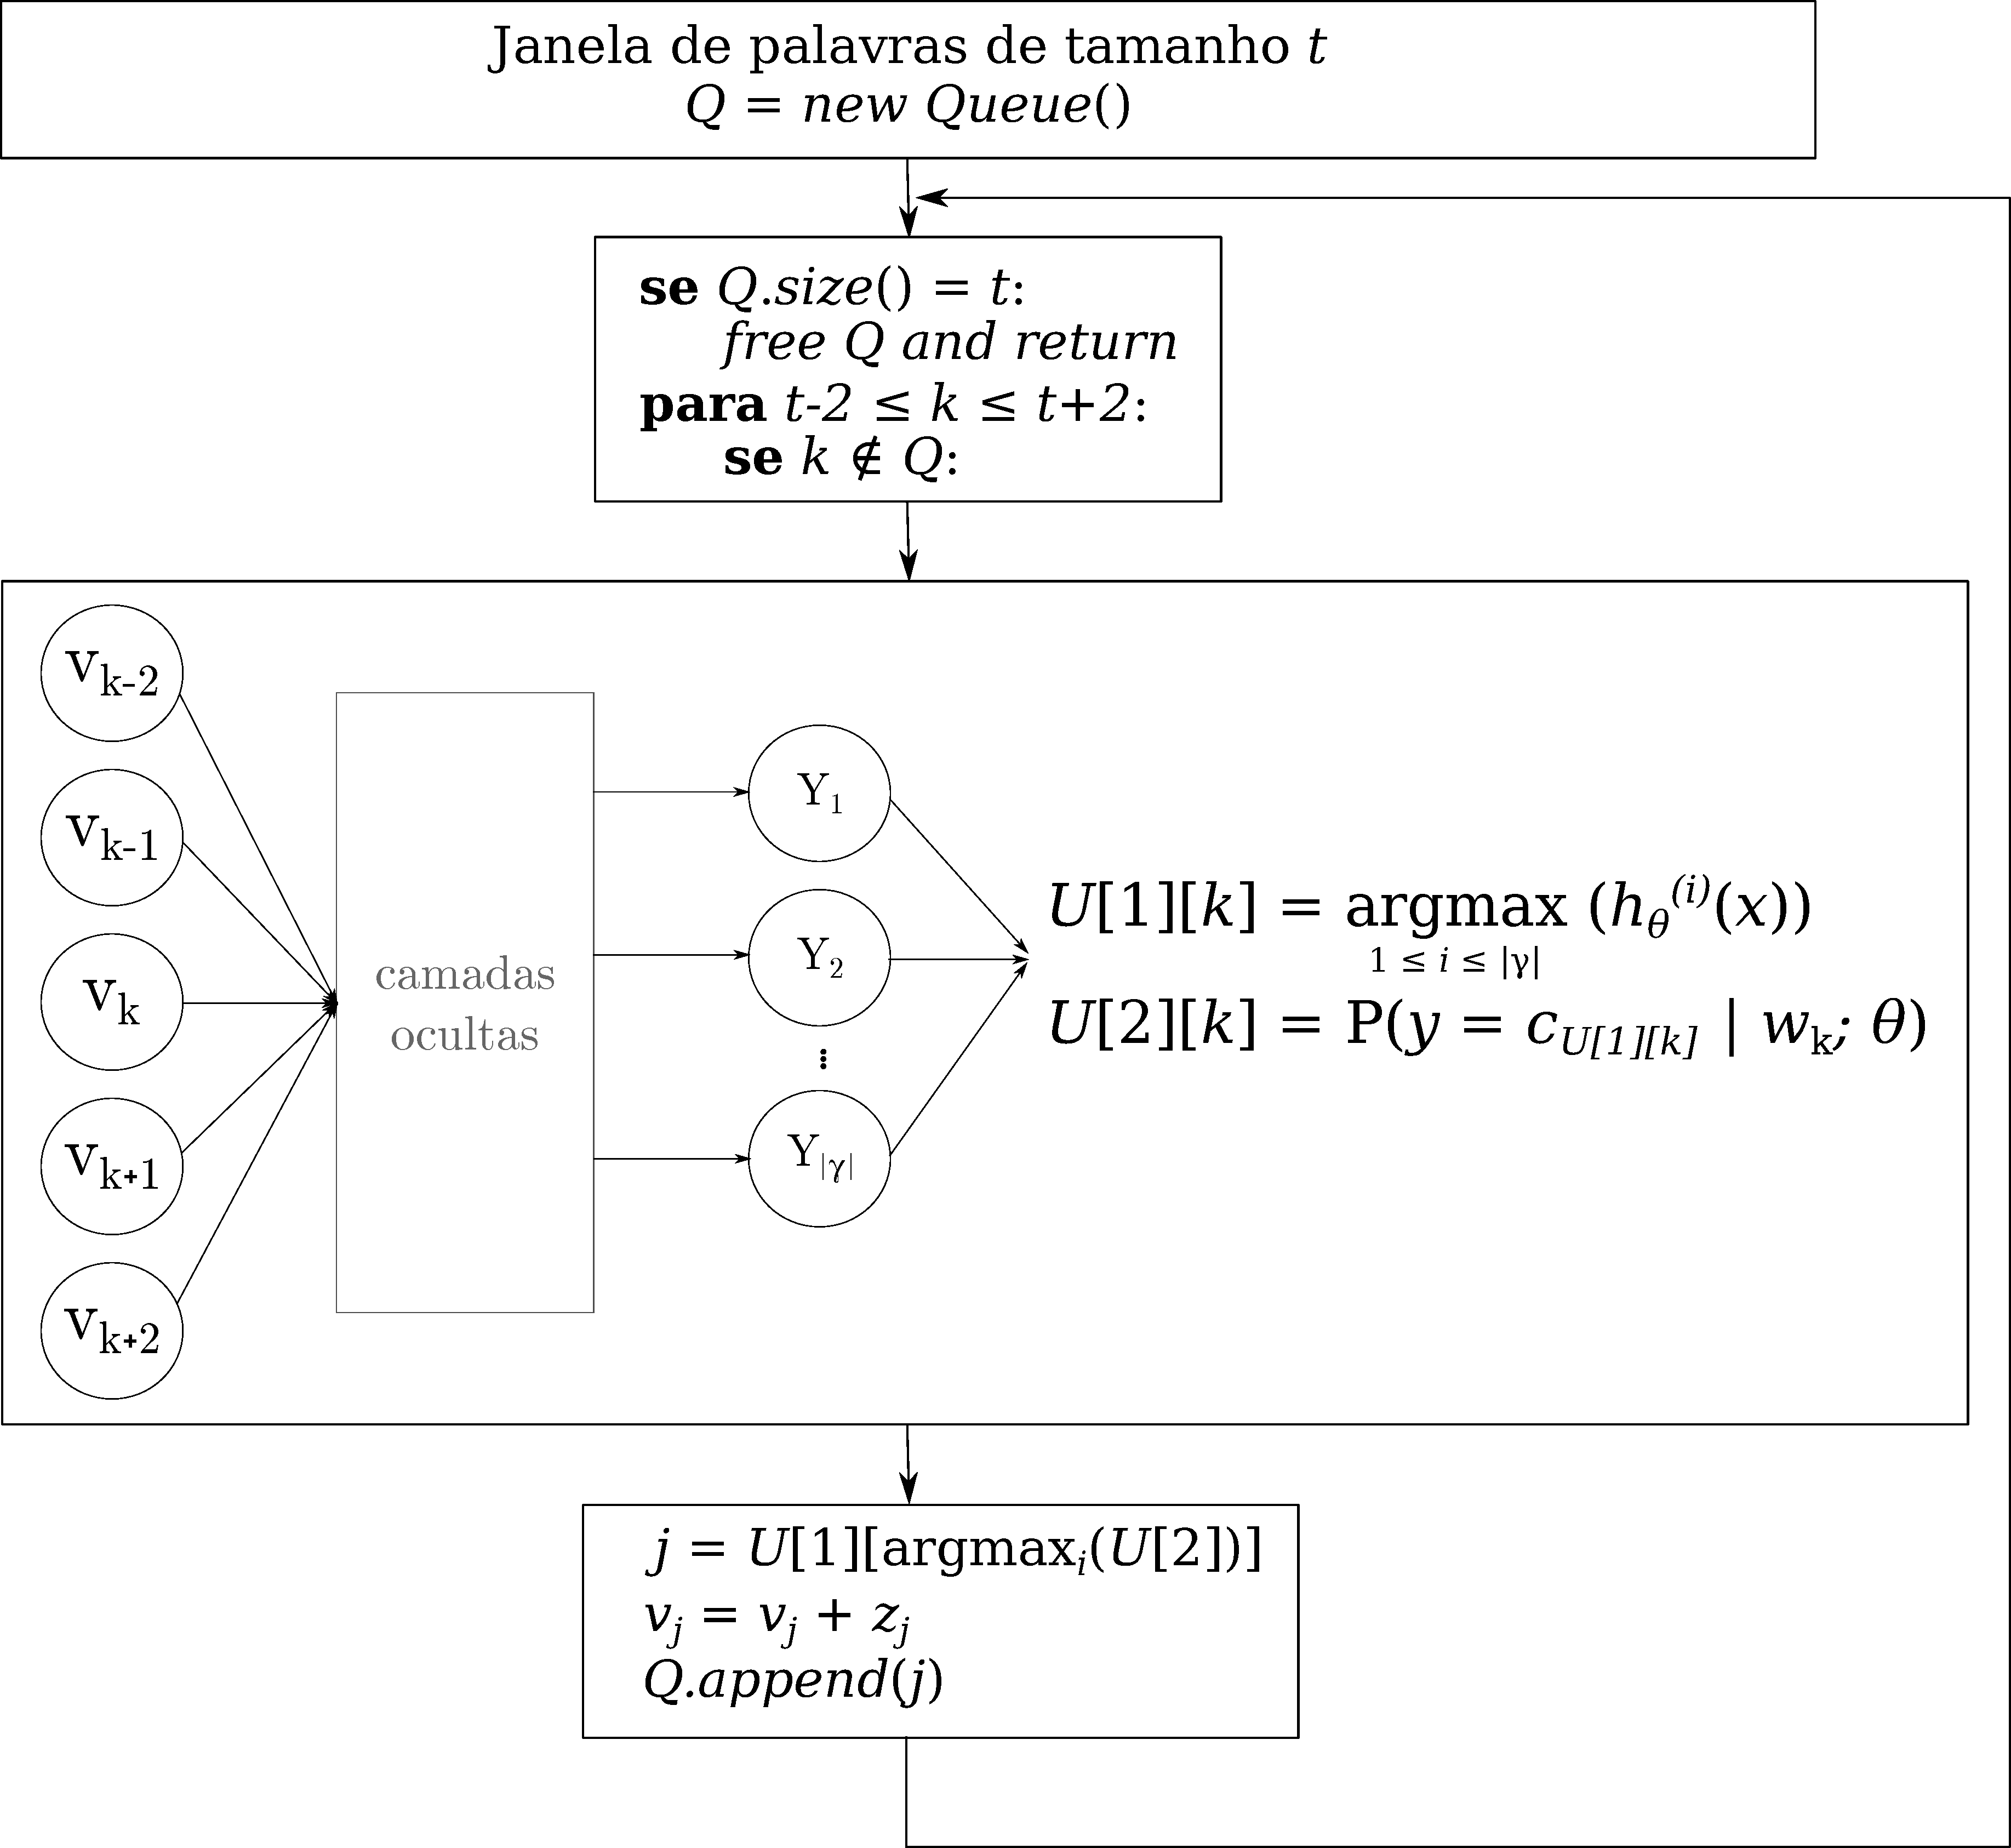
\includegraphics[scale=0.25]{img/neuralnetworkfinal_alg.pdf}
    \end{center}
\end{figure}

Para treinar a rede neural, será seguido uma estratégia de aprendizagem guiada por palavras mais fáceis \cite{shen2007guided}. A \autoref{fig:guidedlearning} exemplifica transições mais fáceis em uma frase, onde o peso mais baixo na aresta representa a ordem de execução. Na verdade, cada transição de um nodo para outro conta como uma nova etapa de treinamento. A \autoref{eq:pontuacaofinal} faz esse aprendizado guiado ao realizar a escolha da palavra mais fácil através da maximização das possibilidades que ainda não foram testadas dentro da janela de palavras.

\begin{figure}[htb]
	  \caption{Grafo de transições de palavras mais fáceis}\label{fig:guidedlearning}
	  \begin{center}
	      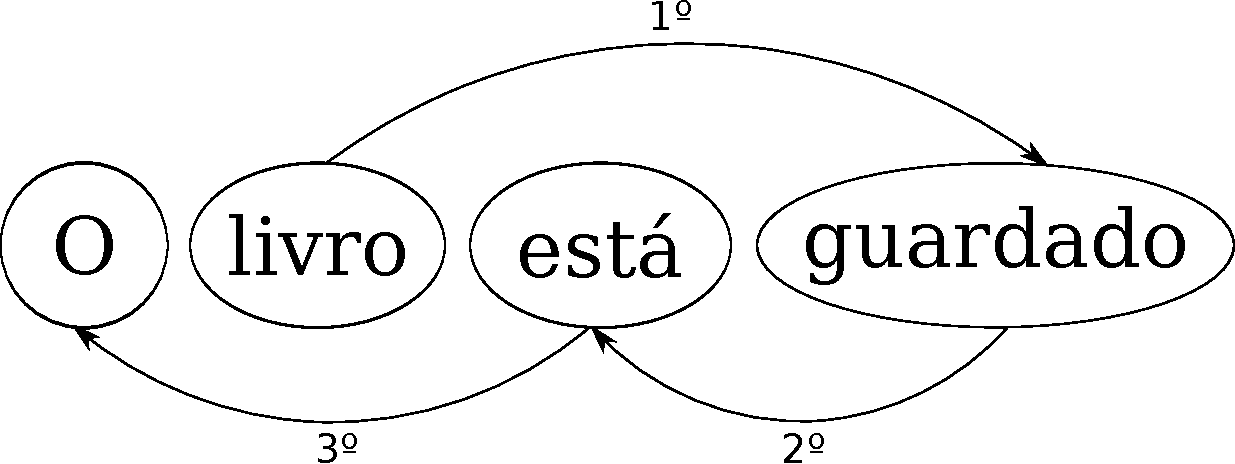
\includegraphics[scale=0.3]{img/guidedlearning.pdf}
	  \end{center}
\end{figure}

Treinar o modelo consiste em ajustar os pesos da rede neural, os valores das \textit{word embeddings} e as pontuações de transição. Após descobrir qual a classe gramatical mais provável para uma palavra $w_n$, o vetor da classe gramatical $z_c$ é composto com o vetor da própria palavra $v_n$ através de uma operação de soma. Essa composição é então armazenada no vetor da própria palavra, conforme mostrado abaixo. 

\begin{equation} \label{eq:composicaovets}
v_n = v_n + z_n
\end{equation}

Na rede neural da \autoref{fig:neuralnetworkfinal}, as camadas ocultas foram removidas da imagem para simplificar a visualização. A saída da rede neural é armazenada num conjunto temporário $U$, que tem duas listas. A primeira lista tem os índices da classe preditada para a palavra sendo analisada $w_k$, já a segunda lista contém as probabilidades da classe preditada ser da palavra $w_k$. Após isso, recupera-se qual a palavra que tem a maior probabilidade de ser classificada. O vetor da classe da palavra recuperada $z_j$ é composto com o vetor da palavra analisada $v_j$ através da \autoref{eq:composicaovets} e o processo se repete até que o conjunto $Q$ tenha tamanho $t$.

Para treinar a rede neural, todos os ajustamentos são feitos em ordem de maximizar a seguinte equação:

\begin{equation}
\sum\limits_{(w_1^t,c_1^t) \in \phi} P(c_1^t|w_1^t,\theta) \nonumber \\
\end{equation}

Onde $\phi$ denota o conjunto dos pares de palavras e classes gramaticais. Computamos a probabilidade acima utilizando uma operação \textit{softmax}:

\begin{align}
P(c_1^t|w_1^t,\theta) = &\ \dfrac{e^{S(w_1^t, c_1^t)}}{\sum\limits_{u_1^t \in \gamma^t} e^{S(w_1^t, u_1^t)}} \nonumber \nonumber \\
log(P(c_1^t|w_1^t,\theta)) = &\ S(w_1^t, c_1^t) - log\Bigg(\sum\limits_{u_1^t \in \gamma^t} e^{S(w_1^t, u_1^t)} \Bigg) \nonumber
\end{align}

A função de custo pode ser definida como:

\begin{equation} \label{eq:costfunctionfinalnn}
J(\theta) = log\Bigg(\sum\limits_{u_1^t \in \gamma^t} e^{S(w_1^t, u_1^t)} \Bigg) - S(w_1^t, c_1^t)
\end{equation}

Onde, há princípio, ajustamos os pesos $\theta$ da rede utilizando o Gradiente Descendente sobre o primeiro termo da função de custo, porém vamos testar com outros algoritmos mais eficientes para essa tarefa, como o Gradiente Descendente Estocástico, Adagrad, Adadelta, etc. \cite{Bengio-et-al-2015-Book}. 

Também queremos maximizar o segundo termo da \autoref{eq:costfunctionfinalnn}. Para isso, seguimos \cite{fonseca2015evaluating} e realizamos um incremento nas pontuações de transição para cada palavra etiquetada em cada etapa do \textit{Backpropagation}, conforme mostrado na equação abaixo:

\begin{equation}\label{eq:gradientsfinalnn}
\frac{\partial J(\theta)}{\partial A_{c_{i-1}, c_{i}, c_{i+1}}} \text{ += } 1 \quad \forall i
\end{equation}


Além disso, incrementamos a função $s_c(v_k) \text{ += } 1$, onde $v_k$ representa a palavra no meio da janela sendo analisada. % [OBRIGATORIO]
%\part{Resultados}
%\input{textuais/outrospontos} % Outro capítulo
%\bookmarksetup{startatroot} % Usar se o próximo capítulo não pertencer à parte anterior e não existir uma parte nova
%==============================================================================
\chapter{Conclusão}\label{conclusao}
%==============================================================================

não tem, só no tcc2! % [OBRIGATORIO]


% +++++++++++++++++++++++++++++++++++++++++++++++++++++++++++++++++++++++++++++++++++++++++++++++++
% ELEMENTOS PÓS-TEXTUAIS
% +++++++++++++++++++++++++++++++++++++++++++++++++++++++++++++++++++++++++++++++++++++++++++++++++
\postextual

% -----------------------------------------------
% Bibliografia [OBRIGATORIO]
% -----------------------------------------------
% Nome(s) do(s) arquivo(s) .bib (sem a extensão)
\bibliography{bibliografia,abntex2-modelo-references}

% -----------------------------------------------
% Apêndices [OPCIONAL]
% -----------------------------------------------
\begin{apendicesenv}

% Imprime uma página indicando o início dos apêndices
\partapendices

% Para cada apêndice, um \chapter


%==============================================================================
\chapter{Derivadas parciais do Gradiente Descendente}\label{app:derivadasgraddesc}
%==============================================================================

De acordo com a ABNT:

\begin{quotation}
Apêndice (opcional): texto utilizado quando o autor pretende complementar sua argumentação. São identificados por letras maiúsculas e travessão, seguido do título. Ex.: APÊNDICE A - Avaliação de células totais aos quatro dias de evolução

Anexo (opcional): texto ou documento \textbf{não elaborado pelo autor} para comprovar ou ilustrar. São identificados por letras maiúsculas e travessão, seguido do título. Ex.: ANEXO A - Representação gráfica de contagem de células
\end{quotation}

Tais definições (e outras) podem ser encontradas na NBR 14724-2001 Informação e documentação - trabalhos acadêmicos\footnote{http://www.firb.br/abntmonograf.htm}.




\end{apendicesenv}


% -----------------------------------------------
% Anexos [OPCIONAL]
% -----------------------------------------------
\begin{anexosenv}

% Imprime uma página indicando o início dos anexos
\partanexos

% Para cada anexo, um \chapter


%==============================================================================
\chapter{Fundamentos de Álgebra Linear}\label{anexo:algebralinear}
%==============================================================================

Sendo anexo, a formatação dessa seção é livre. Ou seja: aceita-se fonte diferente e menor


%==============================================================================
\chapter{LaTex para Principiantes}\label{anexo:latex}
%==============================================================================
TEste\footnote{\cite{Moro2012}}
Dentro dos arquivos .tex o texto pode estar organizado em partes, capítulos, seções, etc. conforme os seguintes comandos:

-- \verb|\part{NomedaParte}|, partes do documento \\
-- \verb|\chapter{Nome}|, capítulos somente para arquivos do tipo \textit{book} e \textit{report}\\
-- \verb|\section{Nome}|, seções\\
-- \verb|\subsection{Nome}|, subseções	\\
-- \verb|\subsubsection{Nome}|, seções dentro de subseções\\
-- \verb|\paragraph{Texto}|, parágrafos formatados	\\
-- \verb|\subparagraph{Texto}|, subparágrafos

\textbf{Parágrafos} Parágrafos são definidos deixando uma linha em branco entre os mesmos.
  Pode-se também forçar usando \verb|\\| bem como deixar uma linha em branco com um \verb|~| sozinho na linha.

\textbf{Formato de texto} O tamanho do texto pode ser definido pelos comandos específicos:  \verb|tiny|,  \verb|scriptsize|,  \verb|footnotesize|, \verb|small|, \verb|normalsize|, \verb|large|, \verb|Large|, \verb|huge| e \verb|Huge|, conforme ilustra a Figura \ref{fig:fontsize}\todo{Perceba que a figura tem resolução ruim; deveria ser uma tabela}.

\begin{figure}[ht]
	\centering
		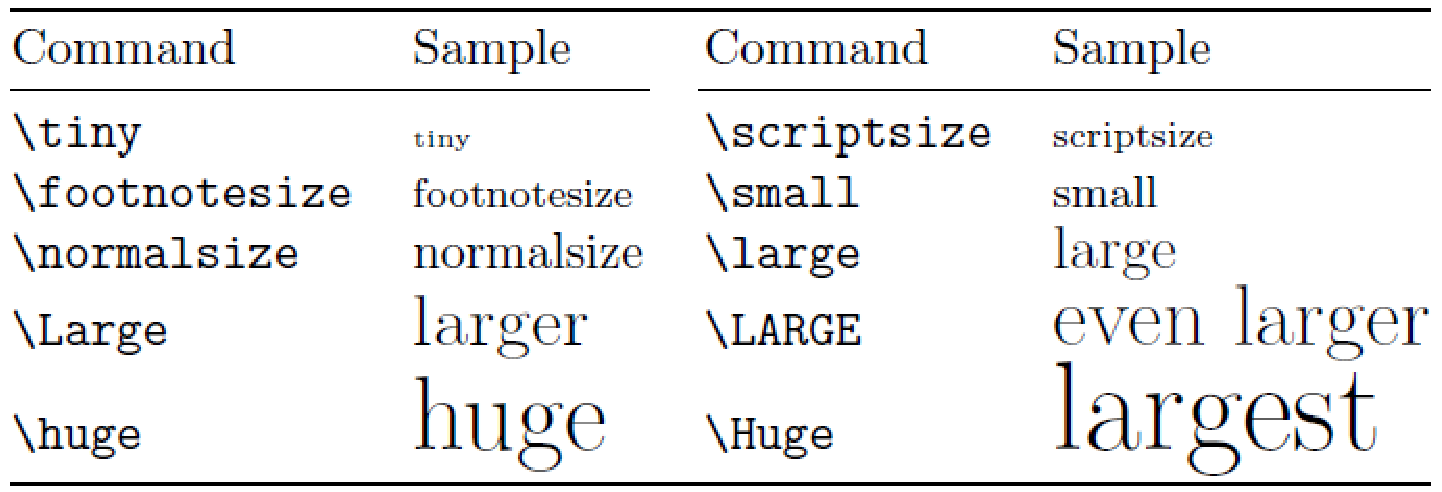
\includegraphics[width=0.7\textwidth]{img/fontsize}
	\caption{Exemplo de tamanhos de fonte}
	\label{fig:fontsize}
\end{figure}

\textbf{Referências dentro do Texto} Partes do texto podem ser referenciadas através do par de comandos \verb|\label| e \verb|\ref|.
  Por exemplo, podemos inserir uma seção no artigo utilizando o seguinte comando:

\begin{verbatim}
\section{Seção principal}\label{sec:prcpal}
\end{verbatim}

Vejam que o título da seção é seguido do comando \verb|\label{nome}|.
  Esta seção pode ser referenciada em qualquer parte do texto, como o exemplo a seguir.

\begin{verbatim}
Conforme explicado na Seção \ref{sec:prcpal}, nosso método utiliza...
\end{verbatim}


%------------------------------------------------------------------------------
\section{Outras Dicas}
%------------------------------------------------------------------------------

\textbf{Caracteres Especiais} Esses não podem ser usados no texto sem a barra à frente: \# \$ \% \^{ } \& \_ \{ \} \~{ } e \slash .

\textbf{Comentários} Comentários são precedidos de \% e podem estar em qualquer parte do texto.
  Lembrando que tudo que estiver após \% será considerado como comentário e ignorado pelo processador.

\textbf{Incluir Figuras} Incluir figuras no LaTeX é relativamente fácil quando se tem um formato de arquivo pré-definido.
  or exemplo, neste documento, usa-se apenas figuras do tipo \textit{pdf}, mas também poderia-se usar do tipo \textit{png} (e \textit{jpeg}, mas este tipo não é recomendado).
  A Tabela \ref{tab:codfig} ilustra as linhas que inserem uma figura no texto. 

\begin{table}[ht]
  \caption{Linhas de código para inserir figura}
	\centering
	\footnotesize	
		\begin{tabular}{l l}
	\\	\hline 
Linha de Código & Explicação \\ \hline 
\verb|\usepackage{graphicx}| & \textit{inclui pacote gráfico no início do documento} \\
\verb|\begin{figure}[tb]|    & \textit{inicia figura, define sua posição no texto} \\
\verb|\centering|            & \textit{centraliza a figura na página}\\
\verb|\includegraphics[scale=.7]|& \textit{define escala da figura}\\
\verb|{img/figura}|      & \textit{inclui o arquivo da figura no texto}\\
\verb|\caption{Legenda}|     & \textit{inclui a legenda da figura}\\
\verb|\label{fig:ap}|        & \textit{inclui o apelido da figura}\\
\verb|\end{figure}|          & \textit{termina figura}\\
		\hline\end{tabular}
	\label{tab:codfig}
\end{table}

\textbf{Hifenização} Às vezes aparece uma palavra cuja hifenização, divisão silábica, está errada. Para resolver esse tipo de problema, pode-se recorrer à divisão manual da palavra, acrescentando \verb|\-| entre cada sílaba: \verb|Mi\-re\-lla|. Se, ao invés desta solução, você quiser evitar completamente que suas palavras sejam divididas, acrescente os dois comandos no início do seu documento (ou seja, antes do \\~\textit{begin\{document\}}).

\begin{verbatim}
  \hyphenpenalty=5000
  \tolerance=1000
\end{verbatim}


\textbf{BibTeX} Para editar facilmente o BibTeX, pode-se utilizar uma ferramenta própria\footnote{Ferramentas para BibTeX: http://dmoz.org/Computers/Software/Typesetting/TeX/BibTeX}. A minha favorita é o JabRef\footnote{JabRef Editor: http://jabref.sourceforge.net/}, ilustrado na Figure \ref{fig:jabref}, porque:

\begin{itemize}\addtolength{\itemsep}{-0.5\baselineskip}
	\item É de graça;
	\item Possui interface gráfica super intuitiva;
	\item Permite importar referências de bases clássicas, como ISI, Medline e RIS;
	\item Permite exportar para diferentes formatos, inclusive para um banco de dados utilizando SQL;
	\item Tem botão para procurar o artigo da respectiva referência e fazer o seu download;
	\item Permite adicionar comentários próprios para cada entrada;
	\item Pode-ser classificar as referências e criar grupos para as mesmas, e muito muito mais.
\end{itemize}

\begin{figure}[tb]
	\centering
		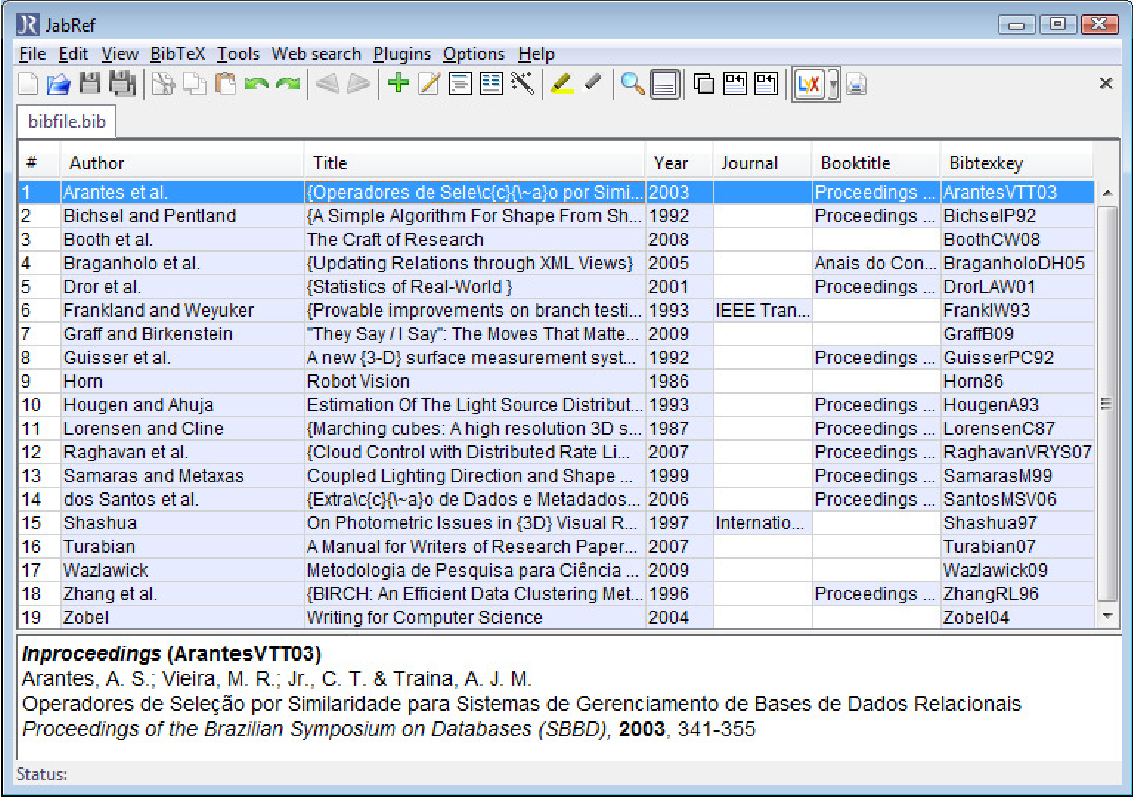
\includegraphics[width=0.98\textwidth]{img/jabref}
	\caption{Tela do JabRef para uma versão inicial do arquivo bib deste documento}
	\label{fig:jabref}
\end{figure}

\textbf{Listas} Listas podem ser definidas com \textit{bullets} ou com números, conforme os exemplos a seguir.

\begin{verbatim}
\begin{itemize}
\item Item 1 com bullet 
\item Item 2 com bullet 
\end{itemize}

\begin{enumerate}
	\item Item 1 numerado
	\item Item 2 numerado
\end{enumerate}
\end{verbatim}

\textbf{Fontes Coloridas} Para adicionar texto em cores (muito útil para marcar trechos do texto que estão \textit{em trabalho}, deve-se adicionar os pacotes \textit{graphicx} e \textit{color} (usando o comando \verb|\usepackage| e depois utilizar o comando \verb|\textcolor{cor}{texto}| para colorir o \textit{texto} com a \textit{cor} especificada. Por exemplo \verb|\textcolor{blue}{texto em azul}|. Outras cores comuns são \textit{red} e \textit{green}.

\textbf{Para Economizar Espaço} Existem alguns \textit{dirty tricks}\footnote{Ou seja, eles irão alterar a formatação dada pelo estilo default do texto.} pra economizar espaço, como por exemplo:

-- \verb|\usepackage{times}| Usa fonte \textit{Times} no lugar da default.

-- \verb|\usepackage[small,compact]{titlesec}| Modifica o título e os espaços antes/depois dos mesmos.

-- \verb|\usepackage[small,it]{caption}| Reduz o tamanho das legendas de tabelas e figuras.

\textbf{WEB} A Web é repleta de páginas e documentos sobre LaTeX. Alguns exemplos incluem:

\begin{itemize}\addtolength{\itemsep}{-0.5\baselineskip}
  \item Favorito inglês: \url{http://en.wikibooks.org/wiki/LaTeX/}
  \item Favorito português: \url{http://linorg.usp.br/CTAN/info/lshort/portuguese/pt-lshort.pdf}
  \item \url{http://www.mat.ufmg.br/~regi/topicos/intlat.pdf}
  \item \url{http://www.duke.edu/~hg9/ctex/LaTeXManual.pdf}
  \item \url{http://minerva.ufpel.tche.br/~campani/cursolatex.pdf}
	\item \url{http://www.personal.ceu.hu/tex/words.htm}
\end{itemize}


\end{anexosenv}


% -----------------------------------------------
% Índice Remissivo [OPCIONAL]
% -----------------------------------------------
% Veja o pacote makeindex para mais informações
\printindex


\end{document}
